\chapter{External Contact Detection from Joint Torque Measurements} \label{chapter:force_from_torque}
\section{Introduction}
No longer confined to factory-floor workcells repeating painstakingly hand-coded trajectories, robot arms today have been tasked with increasingly open-ended assignments such as ``put this shoe on the shelf'' or ``load the dish washer'', where the robots need to operate in unknown, unstructured environments potentially populated by humans. Naturally, the safety of such operations hinges upon the robot's ability to reliably handle unplanned collisions between any part of itself and the environment. 

The ultimate sensor for collision detection is perhaps a sensitive tactile skin covering the entire surface of the robot \cite{cannata2008embedded, jain2013reaching}. However, such skins are rarely seen outside research labs, as they are usually expensive and prone to wear and tear. On the other hand, joint-level proprioceptive torque sensors are mature, robust and becoming more common in robot arms designed for human-robot interactions \cite{loughlin2007dlr, franka}.

Several techniques have been developed to estimate both the external contact force and its location on the whole robot using only proprioceptive torque sensors \cite{haddadin2017robot, manuelli2016localizing, zwiener2018contact, zwiener2019armcl}. However, due to the sparse nature of proprioceptive measurements (one torque measurement per link), estimation of contact force and location from only joint torque has obvious limitations. For a typical serial robot arm with 7 links, when link $i$ (numbered from the base) of the arm is in contact, there are $i$ torque measurements available, and $i \leq 6$ if the contact is not on the end effector. The fact that the contact is pushing the robot gives two additional constraints: the force being in the friction cone and the position being on the robot's surface. In contrast, a contact position has 3 independent components to estimate, and a contact wrench has 6. As a result of this deficiency in available measurements, the literature on joint-torque-based contact estimation commonly assumes that (\textbf{i}) there exists at most one external contact, and (\textbf{ii}) the contact generates negligible moments at the contact point \cite{haddadin2017robot, zwiener2019armcl}.

\begin{figure}
\centering
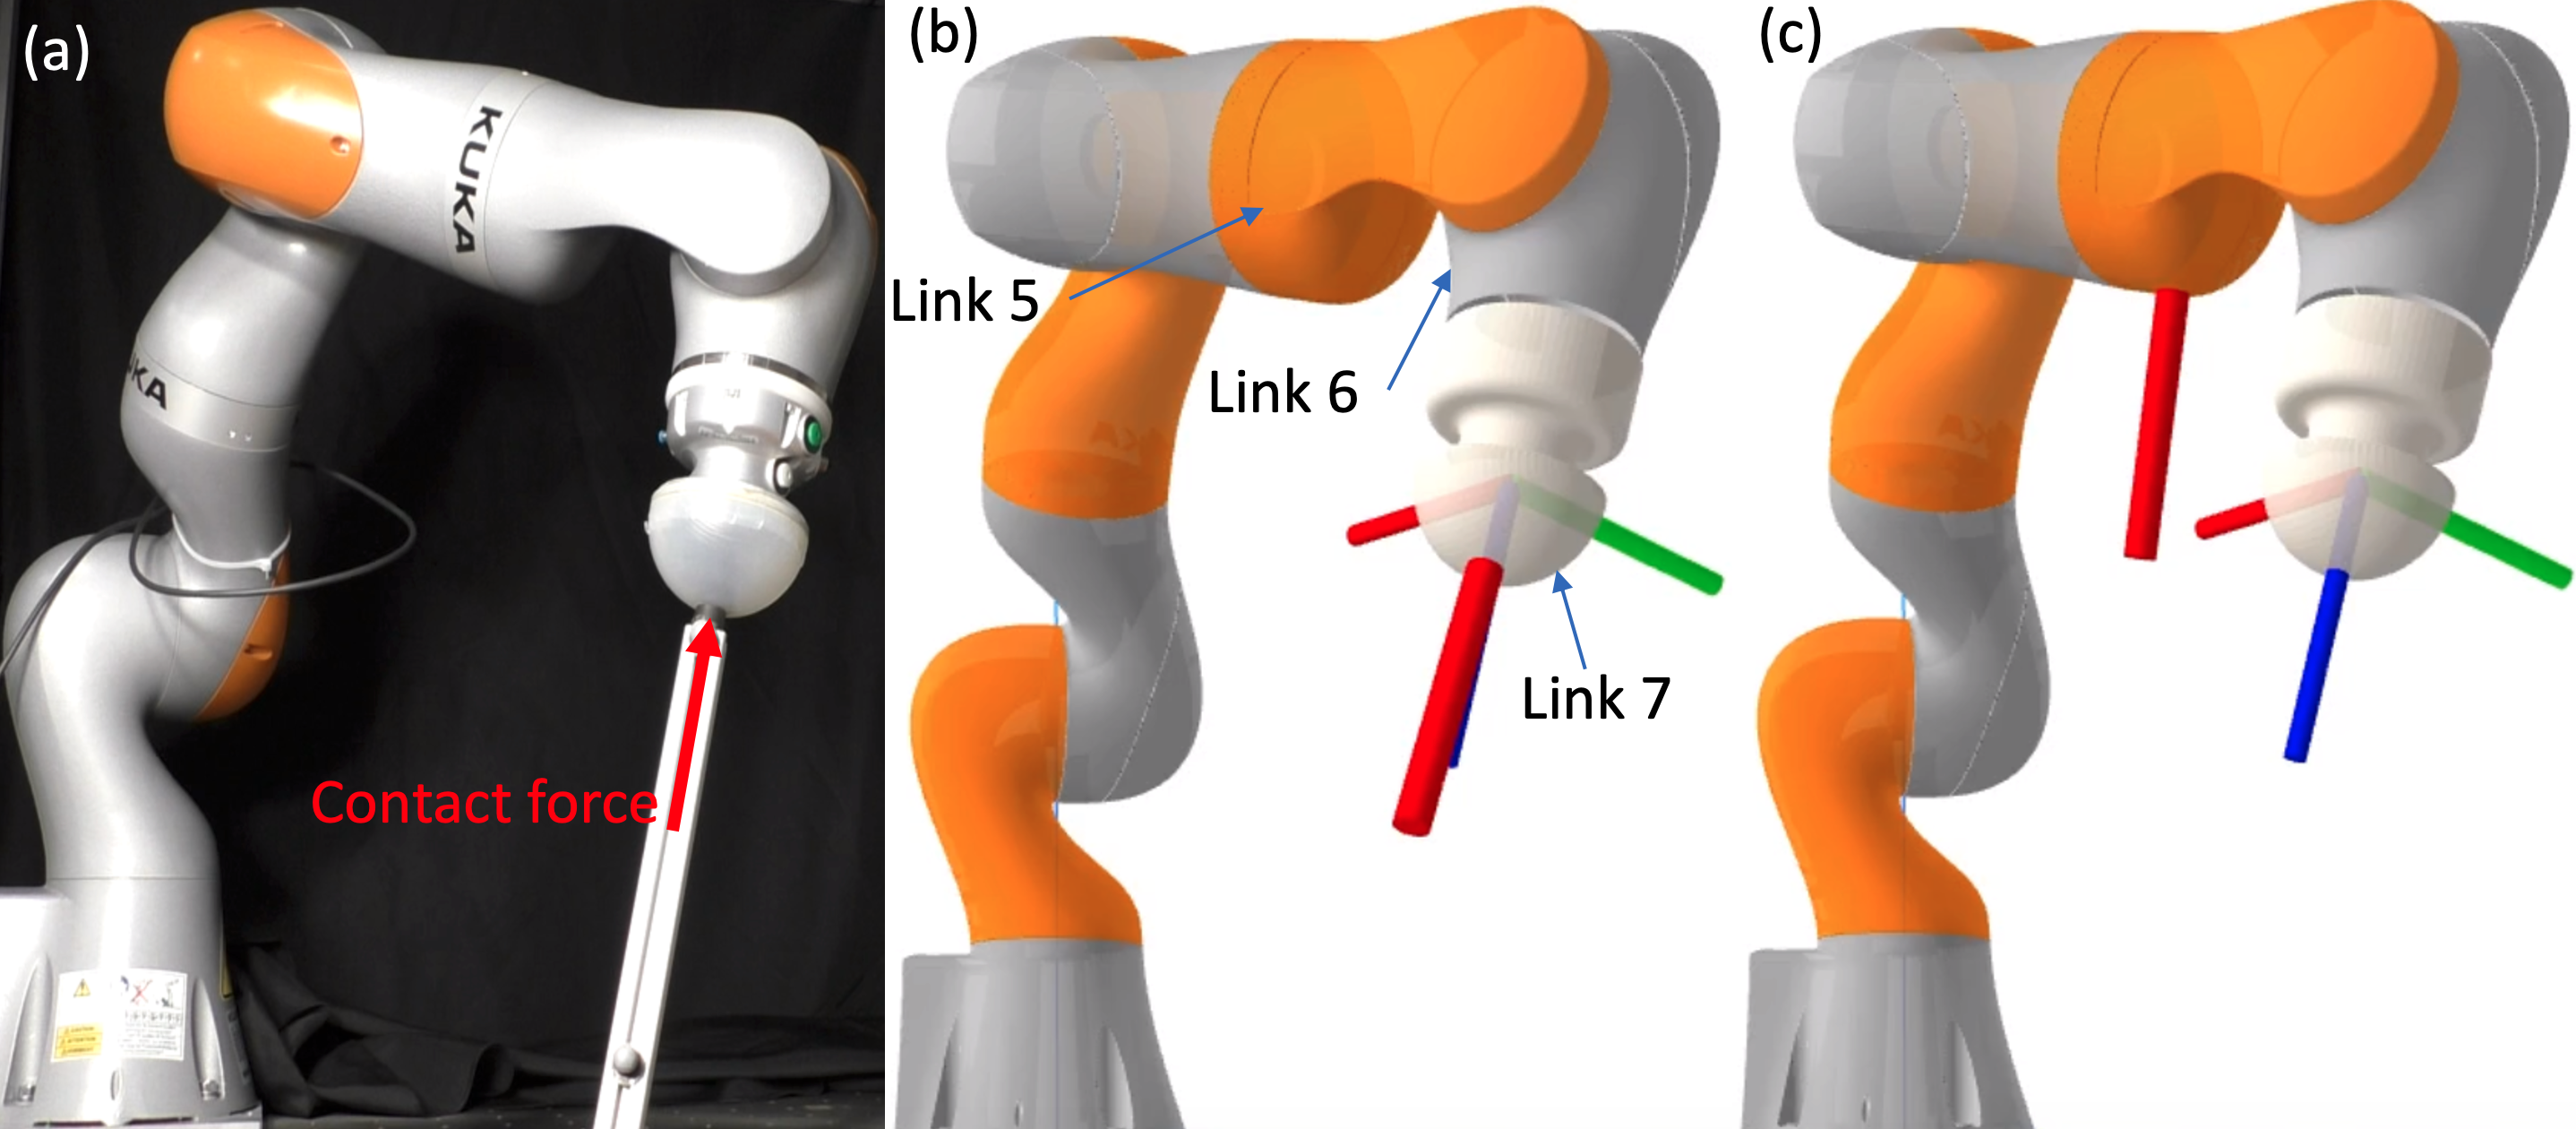
\includegraphics[width=0.9\linewidth]{figures/05_force_from_torque/cpf_failure.png}
\caption{For the true contact shown in (\textbf{a}), which generates little torque about joint 6 and 7, the two contacts in (\textbf{b}) and  (\textbf{c}), represented by red cylinders, create almost identical torque measurements as (\textbf{a}).}
\label{fig:cpf_failure}
\end{figure}

However, even within the boundary set by these simplifying assumptions, joint-torque-based contact estimation is still limited by the loss of detectability of contacts from joint torque measurements, which we will discuss more formally in Section. \ref{sec:observability}. Intuitively, as shown in Fig. \ref{fig:cpf_failure}, it is likely that multiple contact positions and forces (Fig. \ref{fig:cpf_failure}b and \ref{fig:cpf_failure}c) create almost identical torque measurements, making them impossible to distinguish by looking at joint torque alone. Although this failure mode has been observed in existing work \cite{zwiener2018contact}, a thorough analysis on how often joint-torque-based contact estimators fail and what can be done to mitigate such failures appears to be absent from the literature. 

In this chapter, we show quantitatively that two distinct contacts generating almost identical joint torque measurements is far from a 0-probability event. Moreover, this probability can get alarmingly high for links whose geometry is ``concentrated'' around their joint axes, such as links of the IIWA arm. Therefore, we believe that solving for a single contact estimate from joint torque measurements is an inadequate problem formulation. Instead we propose to estimate the \emph{set} of possible contact positions consistent with the measurements.  Elements of this set can be cast as the global optimal solution of a nonlinear optimization problem, which is difficult to solve directly. Nevertheless, by combining rejection sampling and gradient descent on manifolds, we propose an estimator that searches for local minima of the nonlinear optimization problem, and provide an efficient implementation capable of running at real-time rates. In practice, the proposed estimator usually finds all local minima on the links it searches. In addition, given the set of possible contact positions, we also propose an active contact discrimination strategy that falsifies spurious contact positions by slightly moving the robot.


%%%%%%%%%%%%%%%%%%%%%%%%%%%%%%%%%%%%%%%%%%%%%%%%%%%%%%%%%%%%%%%%%%%%%%%%%%%%%%%%
\section{Related Work}
Although raw measurements from joint torque sensors include gravitational and inertial effects, the torque generated by external contacts, also known as the residual torque, can be extracted from them using external torque observers \cite{haddadin2017robot}. Having become an integral part in many robot arms' firmware \cite{loughlin2007dlr, franka}, such observers can update residual torque estimates at hundreds of Hz, providing the foundation for all proprioceptive contact estimation methods.

The contact estimator by Haddadin \textit{et al.} \cite{haddadin2017robot} first determines the link in contact as the last link with non-zero residual torque. It then solves for the line of action of the contact force from a system of linear equations relating torque measurements to the contact wrench. Finally, if the contact geometry of the link is convex, intersecting the line with the link will give two potential contact points, one for pulling and the other for pushing. As contact forces almost always push, the contact point can thus be uniquely determined. However, solving for the line of force action needs at least 6 torque measurements and a full-rank contact Jacobian, which implies this method does not produce any outcome on links more proximal to the base than link 6 or when the robot is close to singular. Moreover, when a link is not convex (e.g. link 5 in Fig. \ref{fig:cpf_failure}), the line of force action may intersect the link at more than two locations, making it impossible to uniquely determine the contact point. Last but not least, when the joint torque signals are noisy, which they always are, it is likely that the computed line of action does not intersect with the link geometry at all, making it impossible to determine the contact location \cite{manuelli2018localizing}.

Methods based on the Markov Chain Monte Carlo (MCMC) methodology \cite{manuelli2016localizing, zwiener2019armcl} can theoretically work on any link and with rank-deficient contact Jacobians, although estimation accuracy typically degrades on links too close to the base, or when the robot is close to singular. The degradation is not a limitation of the methods themselves, but a result of the loss of detectability of contacts from joint torque measurements. Both \cite{manuelli2016localizing} and \cite{zwiener2019armcl} use random walk on the robot's surface as the proposal distribution, and evaluate the likelihood of samples using the L2 norm of the difference between the measured joint torque and the joint torque created by the sample. The difference is that \cite{manuelli2016localizing} assumes frictional contacts whereas \cite{zwiener2019armcl} assumes that contacts are frictionless. The biggest drawback of MCMC methods is that they typically converge to only one local minima of the likelihood function, and are oblivious of other local minima when they exist.

Proprioceptive contact estimator based on machine learning has also been explored. Zwiener \textit{et al.} discretize a robot's surface into finitely many patches, and train a classification network to predict the patch in contact from joint torque \cite{zwiener2018contact}. Although the contact classifier works well on both the training and validation data sets, its limitations and failure modes are difficult to analyze; its ability to generalize beyond the data set it is trained on is also hard to gauge. 

%%%%%%%%%%%%%%%%%%%%%%%%%%%%%%%%%%%%%%%%%%%%%%%%%%%%%%%%%%%%%%%%%%%%%%%%%%%%%%%%
\section{Problem Formulation \label{sec:problem_statement}}
For given joint angles $q \in \mathbb{R}^{n_q}$ and residual joint torque $\tauE \in \mathbb{R}^{n_q}$ created by one external contact at point $C^\star$, the problem is to find $p_{C^\star} \in \mathbb{R}^3$, the coordinate of contact point $C^\star$, and the contact force $f_{C^\star}$. In other words, we would like to solve for $p_{C^\star}$ and $f_{C^\star}$ from the following equation:
\begin{equation}
\label{eq:torque_jacobian_force}
\tauE = \J_C({q}, {p}_C)^\intercal {f}_C,
\end{equation}
where $C$ is a generic point on the robot's surface; $\J_C({q}, {p}_C) \in \mathbb{R}^{3 \times n_q}$ the contact Jacobian that maps joint velocity $\dot{q}$ to the velocity of $C$. 

As shown in Fig. \ref{fig:friction_cone}a, the contact force ${f}_C$ needs to stay inside the friction cone at $C$: $\norm{{f}_{C_f}} \leq \mu \norm{{f}_{C_n}}$. The second-order cone can be approximated with the polyhedral cone in Fig. \ref{fig:friction_cone}b, which is generated by a set of $n_d$ extreme rays 
\begin{equation}
\mb{V}_C = \left[{v}_{C_1}, \dots, {v}_{C_{n_d}}\right] \in \R[3 \times n_d], 
\end{equation}
such that 
\begin{equation}
{f}_C = \sum_{i=1}^{n_d} {v}_{C_i} \beta_i = \mb{V}_C {\beta}   
\end{equation}
where $\beta_i \geq 0 \; \forall i$ \cite{stewart2000implicit}.    

\begin{figure}[h]
\centering
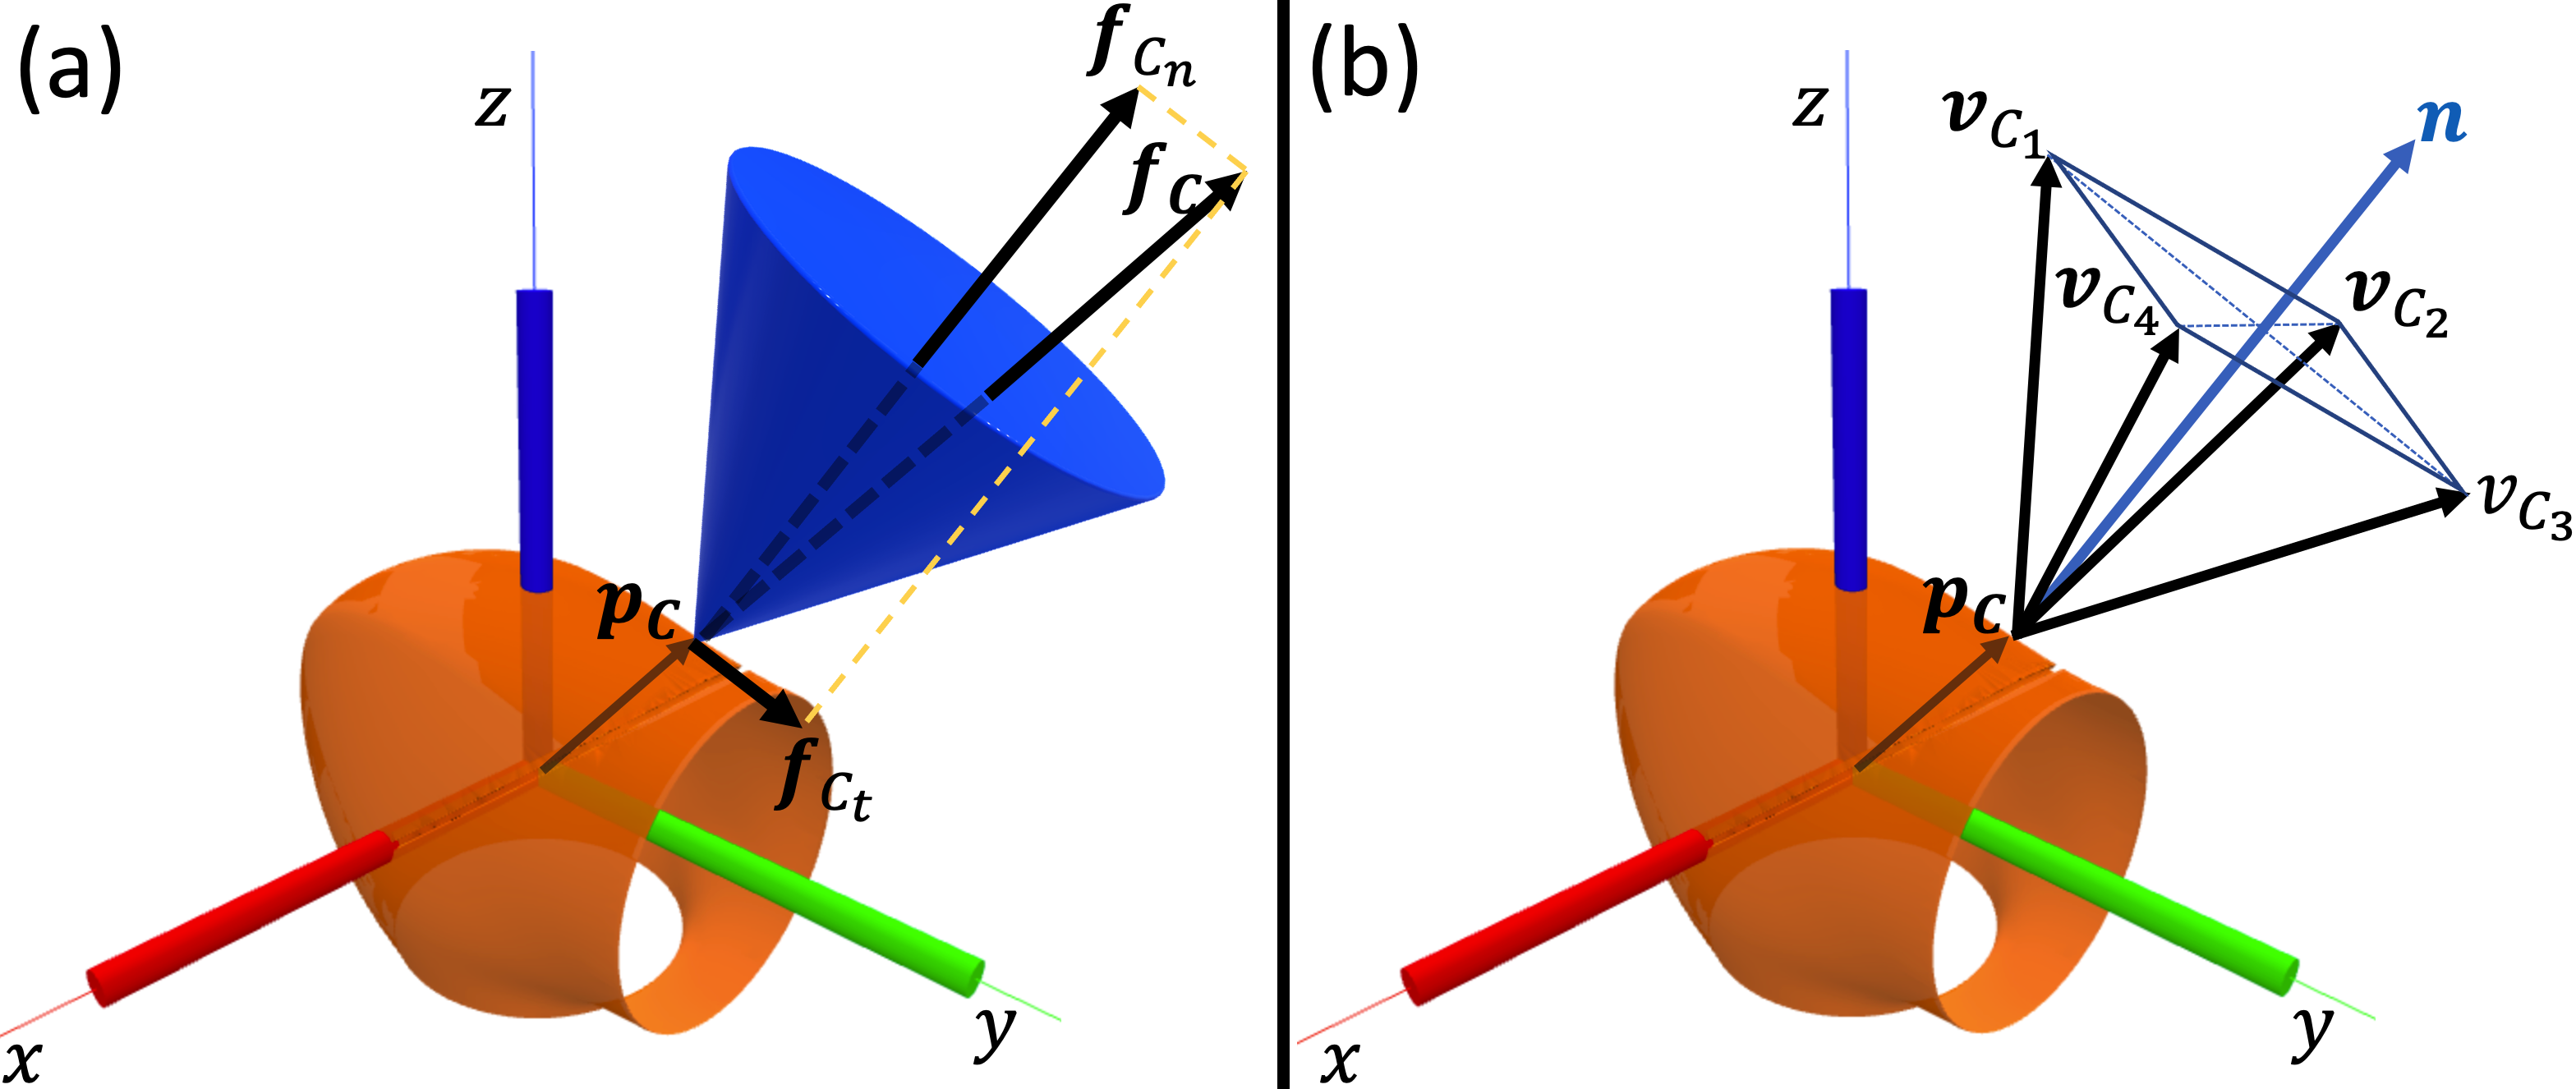
\includegraphics[width=0.98\linewidth]{figures/05_force_from_torque/friction_cone.png}
\caption{A contact force on Link 6 of the KUKA IIWA robot. The orange mesh is the surface of the link. The triad represents the body frame of the link. (\textbf{a}) second-order friction cone. (\textbf{b}) Polyhedral approximation of the friction cone with $n_d=4$.}
\label{fig:friction_cone}
\end{figure}

Solving (\ref{eq:torque_jacobian_force}) with the friction cone constraint is equivalent to solving the following optimization problem:
\begin{equation}
\label{eq:nonlinear_program}
\underset{{\beta} \geq 0, \; \pCbar \in \mathcal{S}}{\text{min.}} \; \| \J({q}, \pCbar)^{\intercal} {\beta} - {\tau}_\text{ext} \|^2,
\end{equation}
where $\J({q}, \pCbar) = \mb{V}_C^\intercal \J_C({q}, \pCbar) \in \mathbb{R}^{n_d \times n_q}$, and $\mathcal{S}$ is the manifold of the robot's surface. For fixed ${q}$ and $\tauE$, a contact position estimate $\pCbar$ has an associated cost defined as
\begin{subequations}
\label{eq:residual_qp}
\begin{align}
l(\pCbar; {q}, \tauE) \coloneqq& \underset{{\beta} \geq 0}{\text{min.}} \; \| \J({q}, \pCbar)^{\intercal} {\beta} - {\tau}_\text{ext} \|^2 \\
=& \underset{{\beta} \geq 0}{\text{min.}} \left({\beta}^\intercal \underbrace{\J\J^\intercal}_{\mathbf{Q}} {\beta} - 2 \left(\underbrace{\J \tauE}_{-{b}}\right)^\intercal {\beta} + \tauE^\intercal \tauE \right). \label{eq:residual_qp:qp}
\end{align}
\end{subequations}
The function $l(\; \cdot \;; {q}, \tauE): \mathbb{R}^3 \rightarrow \mathbb{R}$ is also called the \textit{residual}, and can be computed by solving (\ref{eq:residual_qp:qp}), which is a convex QP. Using $l(\cdot)$, the set of solutions of (\ref{eq:nonlinear_program}) can be described by the set
\begin{equation}
P_0(q, \tauE) \coloneqq \{\pCbar \in \mathcal{S} : l(\pCbar; q, \tauE) = 0\}.
\end{equation}

The true contact location ${p}_{C^\star}$ is clearly in $P_0(q, \tauE)$. However, $P_0$ can have many or even a continuum of elements, i.e. different contact forces at different positions can generate the same joint torque $\tauE$, as shown in Fig. \ref{fig:multiple_local_minima}. In general, it is not possible to distinguish ${p}_{C^\star}$ from other elements of $P_0(q, \tauE)$ using only $q$ and $\tauE$.

\begin{figure}[h]
\centering
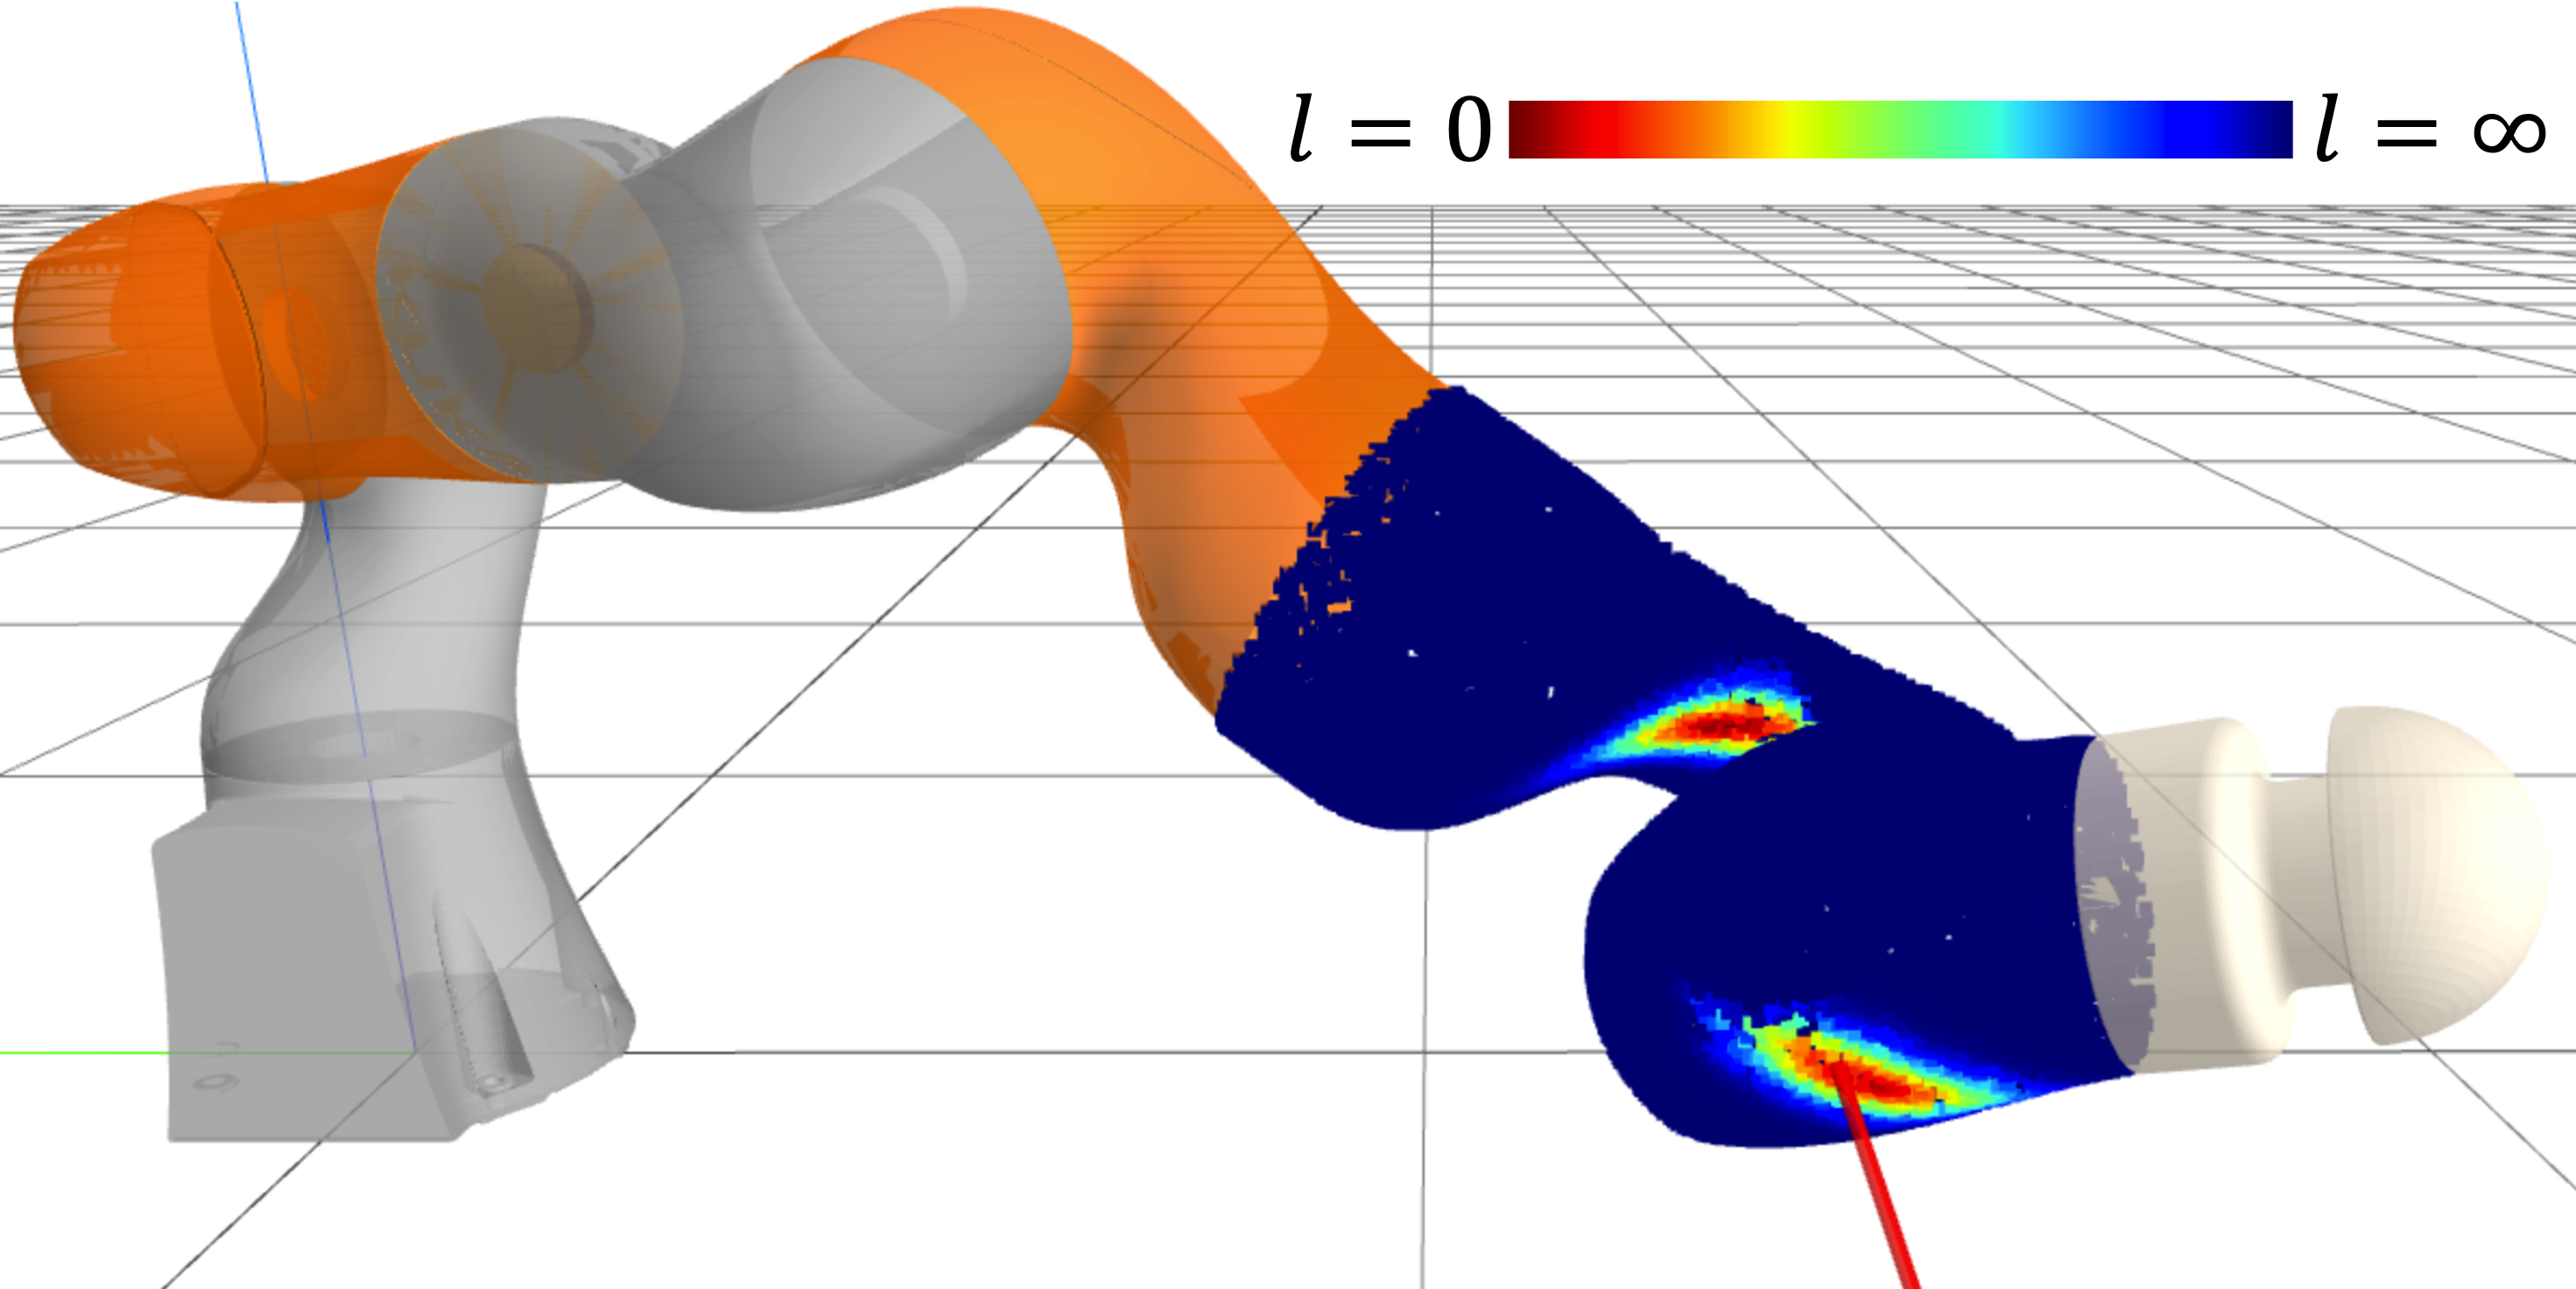
\includegraphics[width=0.85\linewidth]{figures/05_force_from_torque/multiple_local_minima.png}
\caption{The residual $l(\cdot)$ for 20000 sampled points on link 5 and 6 of the IIWA arm. The true contact position and direction is indicated by the red line. Multiple global minima of $l(\cdot)$ can be found on the robot's surface $\mathcal{S}$.}
\label{fig:multiple_local_minima}
\end{figure}

%%%%%%%%%%%%%%%%%%%%%%%%%%%%%%%%%%%%%%%%%%%%%%%%%%%%%%%%%%%%%%%%%%%%%%%%%%%%%%%%
\section{Detectability of contacts \label{sec:observability}}
The joint torque sensor of a link is only able to measure the torque about the axis of the link's revolute joint. It is therefore possible for the torque sensor to register zero or small torque measurement, even if the link is in contact with significant contact force. In this section, we give a quantitative analysis on how likely a contact force creates little or no measurable torque by studying the simplest case of a single link.

\subsection{Detectability}
We assume that a link's joint axis is aligned with the z-axis of the link's body frame. Let $\pC \in \mathcal{S}$ denote a generic point on the robot's surface, $\mathcal{K}_C$ the friction cone at $\pC$, and $\tau_z(\cdot): \mathbb{R}^3 \rightarrow \mathbb{R}$ the function that returns the z-component of the torque generated by a force. For illustrative purposes, the friction coefficient $\mu$ is set to 1. We call the contact at $\pC$ \textit{fully detectable}\footnote{The term ``detectable'', which is rigorously-defined in control theory, is abused in this section in order to facilitate exposition.} if $\forall \fC \in \mathcal{K}_C$, $\norm{\fC} \neq 0 \Rightarrow \tau_z(\fC) \neq 0$. Similarly, the contact is \textit{partially detectable} if $\exists \fC \in \mathcal{K}_C$,  $\norm{\fC} \neq 0 \Rightarrow \tau_z(\fC) \neq 0$, and \textit{undetectable} if $\forall \fC \in \mathcal{K}_C$, $\tau_z(\fC) = 0$.

We first look at the condition under which a contact at $\pC$ is fully detectable. A non-zero force at $\fC$ satisfies $\tau_z(\fC) = 0$ if and only if its line of action intersects with the z-axis. The set of such $\fC$'s belong to the plane which passes through both $\pC$ and the z-axis. We denote this plane by $\mathcal{P}_C$. The contact at $\pC$ is fully detectable if and only if $\mathcal{K}_C \cap \mathcal{P}_C = \{{0}\}$, which is equivalent to the following linear program being infeasible:
\begin{subequations}
\label{eq:find_min_torque}
\begin{align}
\text{Find} \; {\beta}, \; \text{subject to} &  \\
\left(\pC \times {e}_z\right)^\intercal \left(\mb{V}_C {\beta} \right) &= 0, \label{eq:find_min_torque:plane}\\
{\beta} &\geq 1, \label{eq:find_min_torque:non-zero}
\end{align}
\end{subequations}
where ${e}_z$ is the unit vector along the z-axis; $(\pC \times {e}_z)$ is normal to $\mathcal{P}_C$. (\ref{eq:find_min_torque:plane}) constrains the contact force $\fC = \mb{V}_C {\beta}$ to $\mathcal{P}_C$. (\ref{eq:find_min_torque:non-zero}) makes sure that $\fC$ is non-zero. 

To find out which part of a link is fully detectable, we can sample uniformly on the link's surface and solve (\ref{eq:find_min_torque}) for all samples. The results for two links with distinct geometries are shown in Fig. \ref{fig:full_observability}. As the IIWA link's surface is ``concentrated'' around its joint axis, only a tiny fraction of the link's surface is fully detectable. In contrast, the ``elongated'' link of UR5 has significantly more fully detectable surface, which is located further away from the joint axis. On both links, the majority of the samples are not fully detectable. 
\begin{figure}[h]
\vspace{-0.2cm}
\centering
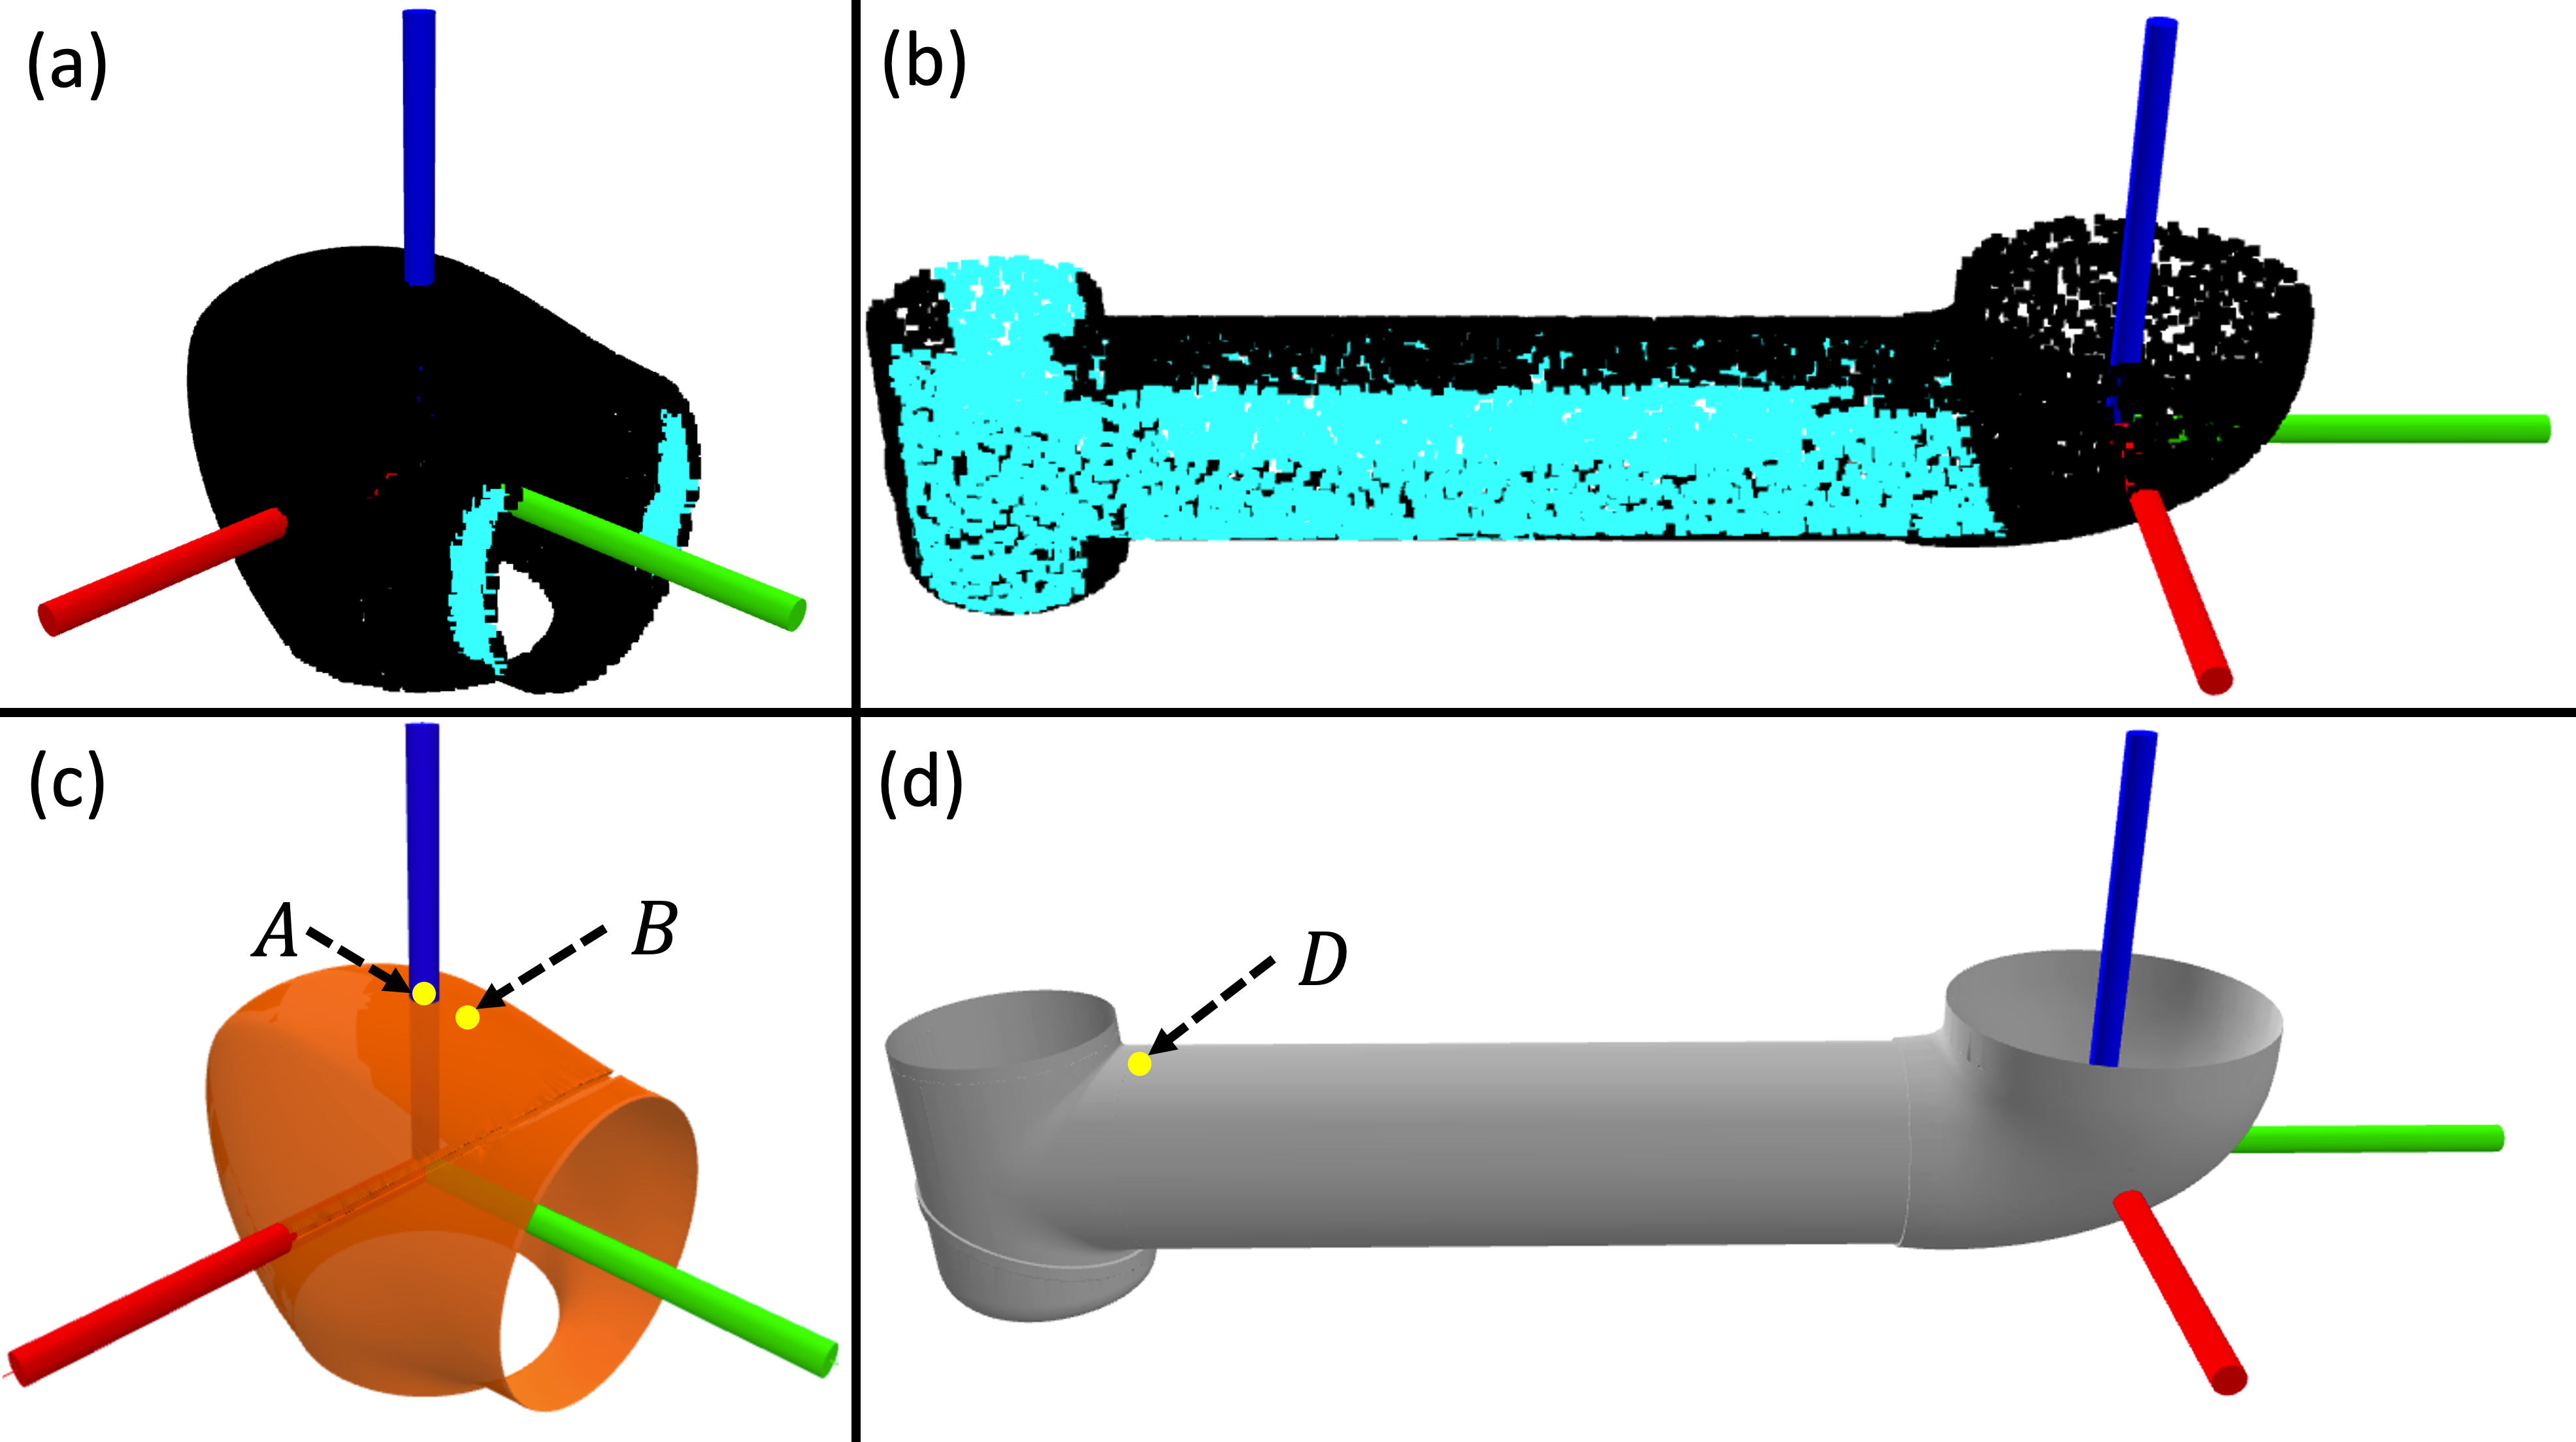
\includegraphics[width=\linewidth]{figures/05_force_from_torque/full_observability.png}
\caption{Full detectability of (\textbf{a}) link 6 of the IIWA arm and (\textbf{b}) ``forearm'' link of the UR5 arm. Out of the 20000 samples generated on each link, 2.19\% and 32.58\% of the samples on (\textbf{a}) and (\textbf{b}) are fully detectable, respectively. Fully detectable samples are shown in cyan, others in black. The meshes of the links are shown in (\textbf{c}) and (\textbf{d}). Points $A$, $B$ and $D$ are examples of different levels of detectability, which will be defined in Sec. \ref{sec:undetectability}.}
\label{fig:full_observability}
\vspace{-0.5cm}
\end{figure}

\subsection{Quantifying ``undetectability''} \label{sec:undetectability}
A contact at $C$ is fully detectable if any contact force in $\mathcal{K}_C$ generates \textit{any} non-zero torque measurement. However, as real torque sensor measurements are usually corrupted by noise, it is useful to know when a contact force generates a torque measurement no less than a threshold $\epsilon$.

Moreover, for contacts that are not fully detectable, it is worth noting that the extent of their ``undetectability'' varies. For example, point $A$ in Fig. \ref{fig:full_observability}c is undetectable, as it is the intersection of the z-axis and the link's surface. Although both point $D$ (Fig. \ref{fig:full_observability}d) and $B$ (Fig. \ref{fig:full_observability}c) are partially detectable, it generally takes a smaller force to generate $\tau_z > \epsilon$ at $D$ than at $B$, as $D$ is further away from its joint axis.

The degree of a contact's ``undetectability'' with respect to the threshold $\epsilon$ can be quantified by:
\begin{subequations}
\begin{align}
\eta_\epsilon(\pC) &\coloneqq \frac{\text{Area}(\mathcal{D}_c^\epsilon)}{\text{Area}(\mathcal{D}_c)} \in [0, 1],  \\
\mathcal{D}_C &\coloneqq \{\fC \in \mathbb{R}^2 : \norm{\fC} = 1, \fC \in \mathcal{K}_C\}, \\
\mathcal{D}_C^\epsilon &\coloneqq \{\fC \in \mathcal{D}_C : \tau_z(\fC) \leq \epsilon \}, 
\end{align}
\end{subequations}
where $\mathcal{D}_C$ is a ``dome'' in the friction cone consisting of unit-norm forces, and $\mathcal{D}_C^\epsilon$ is the subset of $\mathcal{D}_C$ consisting of forces whose torque measurement $\tau_z(\fC)$ is less than $\epsilon$. Intuitively, $\eta_\epsilon(\pC)$ is the proportion of contact forces in $\mathcal{K}_C$ that create small ($\leq \epsilon$) torque measurements. The closer $\eta(\pC)$ is to 1, the less detectable $\pC$ becomes. Using Fig. \ref{fig:full_observability}c and \ref{fig:full_observability}d again as examples, we expect $\eta_\epsilon({p}_A) = 1$, $\eta_\epsilon({p}_B)$ be close to 1, and $\eta_\epsilon({p}_D) < \eta_\epsilon({p}_B)$. 

Computing $\eta_\epsilon(\pC)$ can be done analytically, but a sampling based approach is much easier to implement. Uniform samples on $\mathcal{D}_C$ can be easily generated, and checking membership of $\mathcal{D}_C^\epsilon$ is trivial. We can then approximate $\eta_\epsilon(\pC)$ by the ratio of samples in $\mathcal{D}_C^\epsilon$ to the total number of samples.

To evaluate the ``undetectability'' of an entire link, we can once again compute $\eta_\epsilon(\cdot)$ for samples generated uniformly from the link's surface. The results for two different links using different $\epsilon$'s are summarized in Fig. \ref{fig:partial_observability}. As $\epsilon$ increases, the surface close to the z-axis quickly becomes fully undetectable. If we treat $\epsilon$ as a detection threshold, the result becomes particularly alarming for links with a more ``concentrated'' shape: even for $\epsilon=0.02$ (Fig. \ref{fig:partial_observability_eisilon_0.02}): $\eta_\epsilon \geq 0.4$ for 80\% of the samples. In other words, if a force of $1\mathrm{N}$ is applied at a random point $C$ along a random direction in $\mathcal{K}_C$, the probability of not detecting the contact force is at least 0.32.

\begin{figure}
\centering
\subfloat[$\epsilon$=0.02. IIWA: $\eta_{\text{min}}=0.011, \eta_{\text{max}}=1$. UR5: $\eta_{\text{min}}=0, \eta_{\text{max}}=1$.]{
	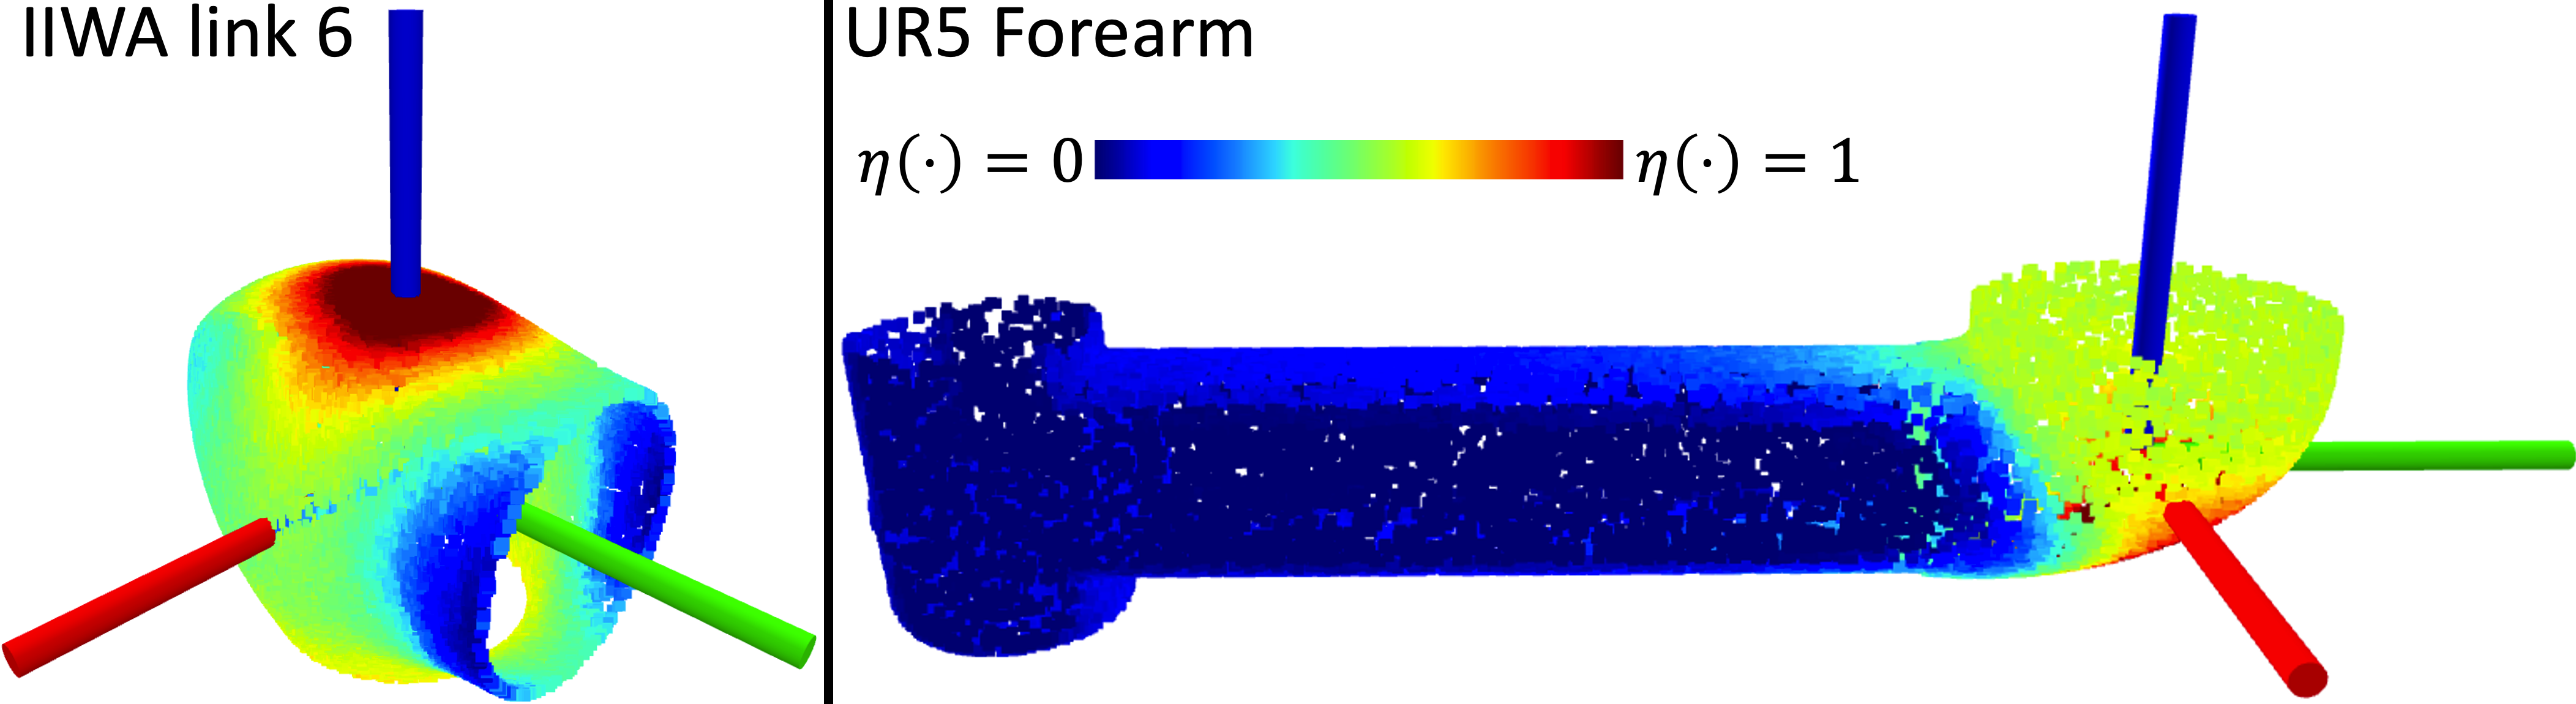
\includegraphics[width=0.97\linewidth]{figures/05_force_from_torque/partial_observability_eisilon_0.02.png}
	\label{fig:partial_observability_eisilon_0.02}
}\\
\subfloat[$\epsilon$=0.05. IIWA: $\eta_{\text{min}}=0.249, \eta_{\text{max}}=1$. UR5: $\eta_{\text{min}}=0, \eta_{\text{max}}=1$.]{
	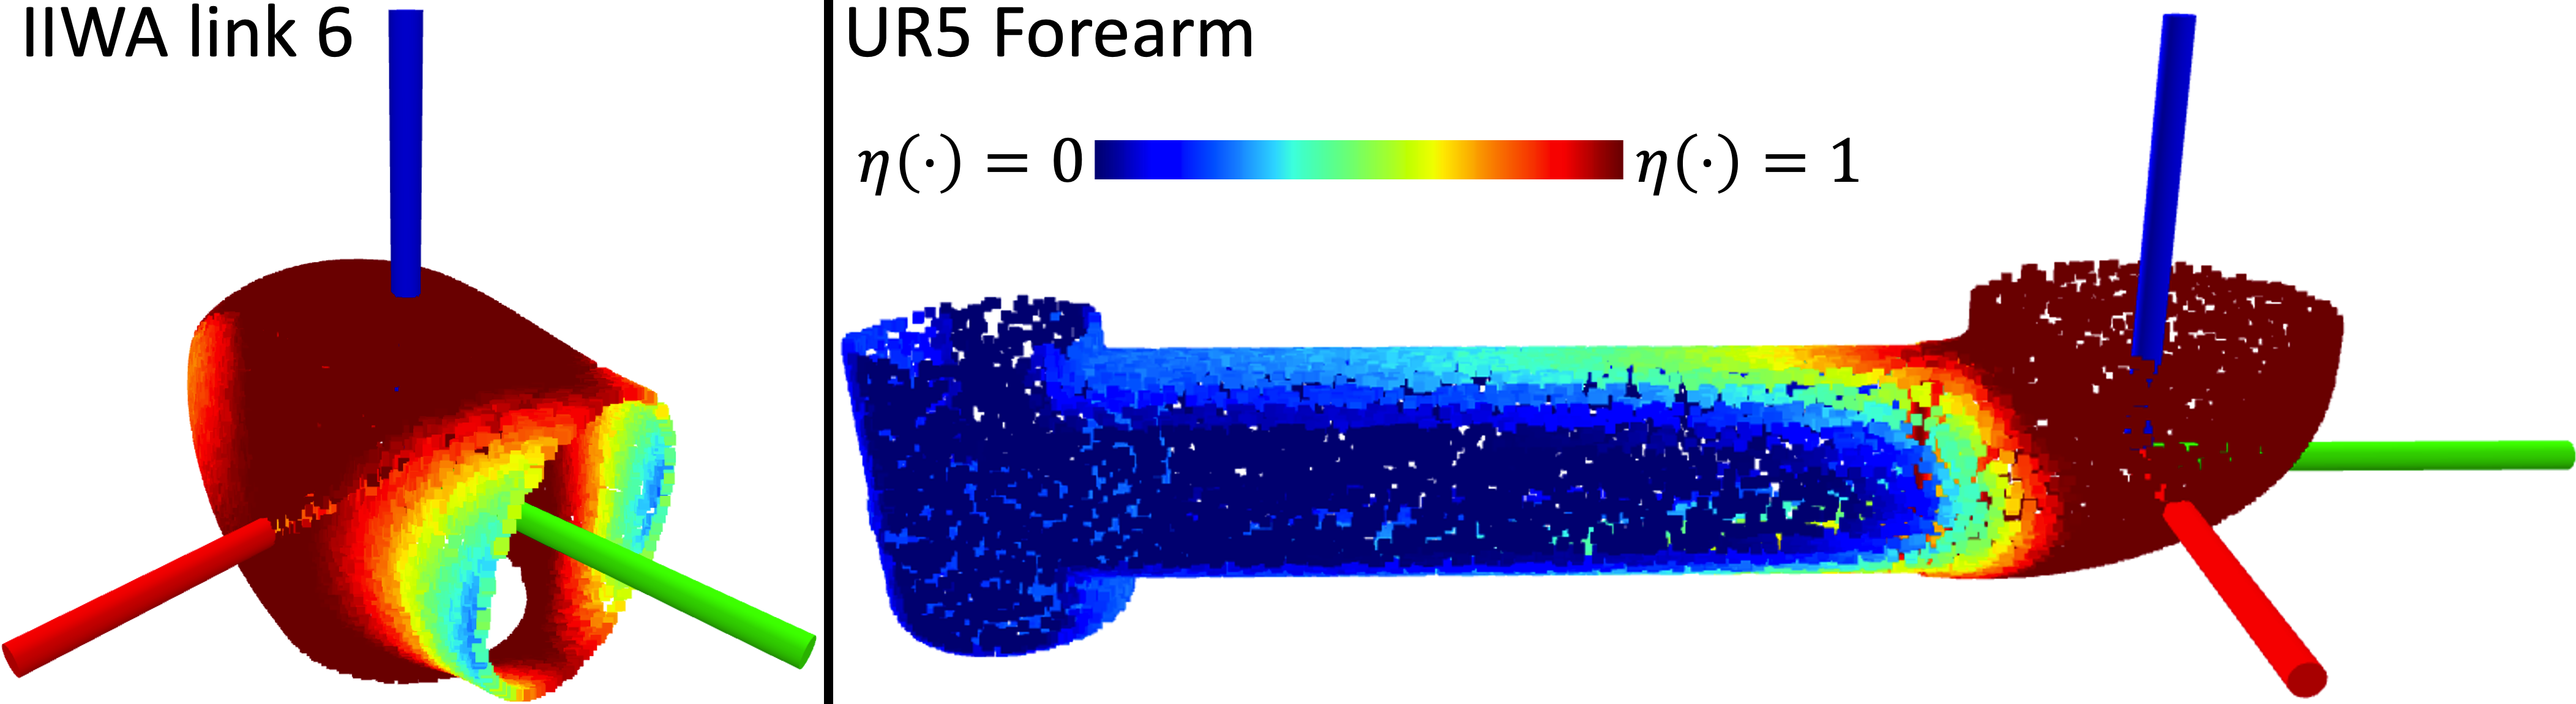
\includegraphics[width=0.97\linewidth]{figures/05_force_from_torque/partial_observability_eisilon_0.05.png}
	\label{fig:partial_observability_eisilon_0.05}
}\\
\subfloat[$\epsilon$=0.1. IIWA: $\eta_{\text{min}}=1, \eta_{\text{max}}=1$. UR5: $\eta_{\text{min}}=0, \eta_{\text{max}}=1$.]{
	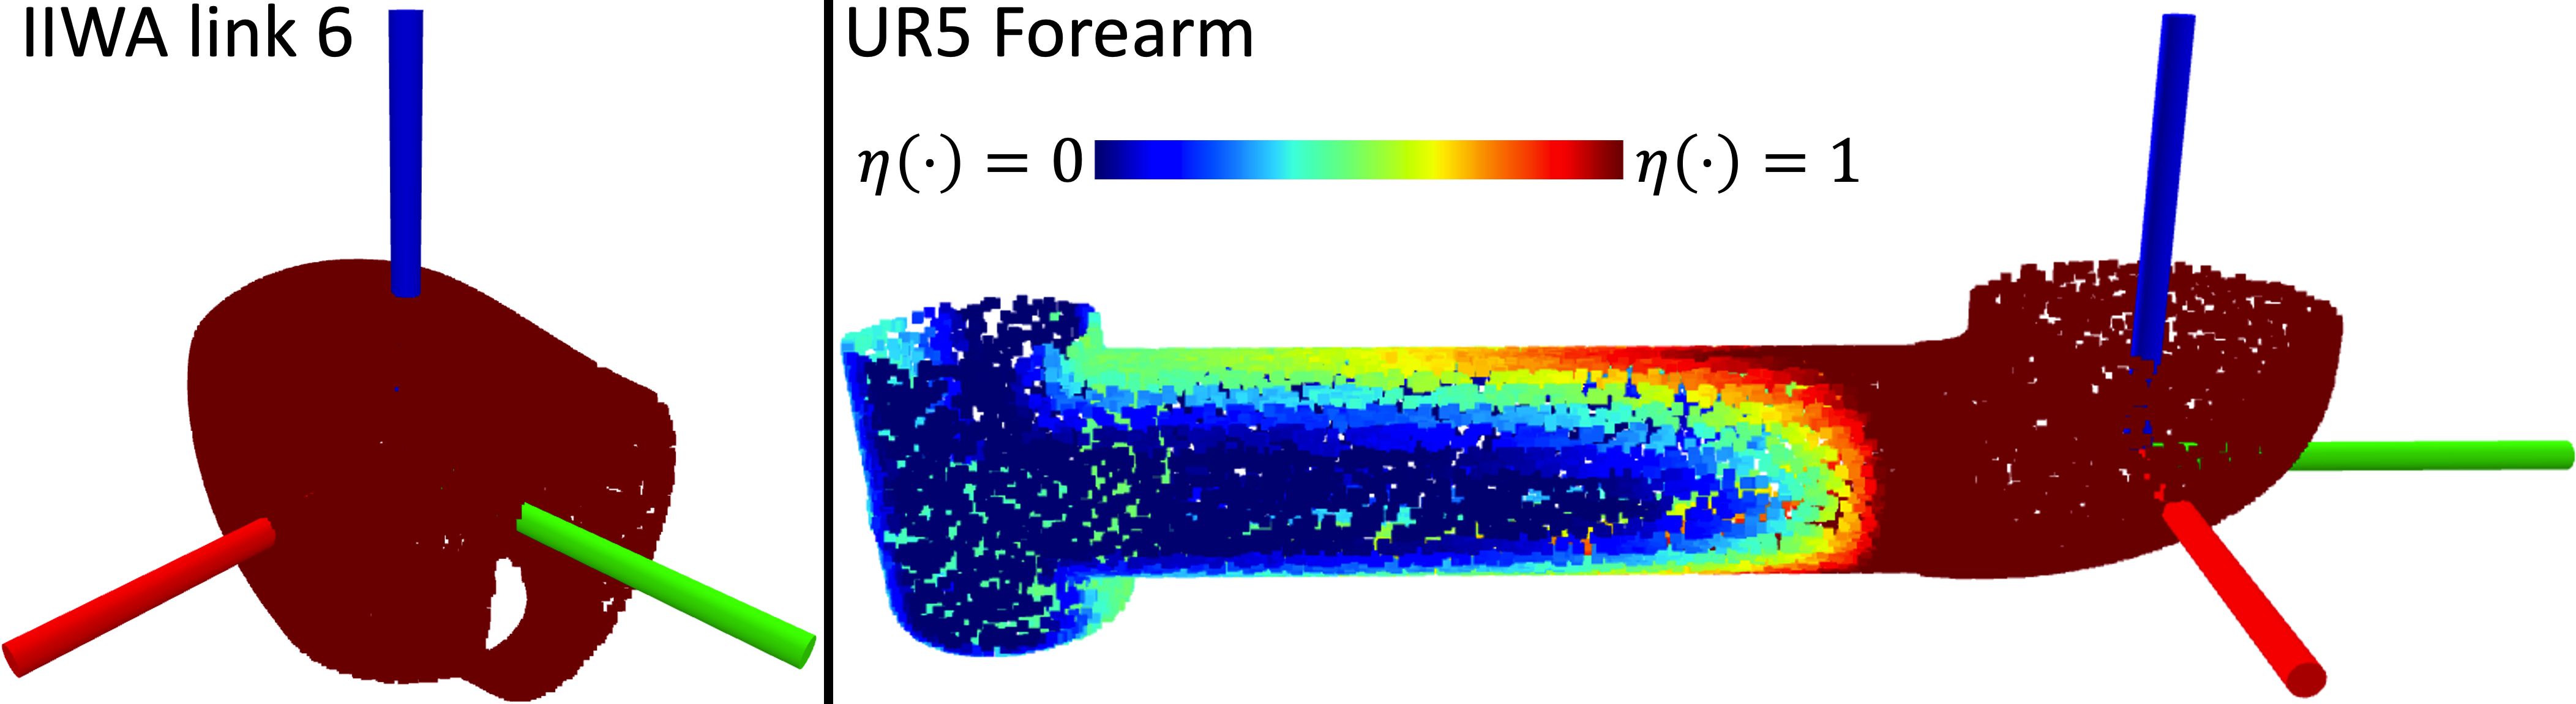
\includegraphics[width=0.97\linewidth]{figures/05_force_from_torque/partial_observability_eisilon_0.1.png}
	\label{fig:partial_observability_eisilon_0.1}
}
\caption{$\eta_\epsilon(\cdot)$ of IIWA link 6 and UR5 forearm. }
\label{fig:partial_observability}
\end{figure}

\subsection{Implications}
The analysis in this section reveals a fundamental limitation of existing joint-torque-based contact estimation methods: when a contact force generates small torque about the axis of a link, the observed $\tauE$ could be equally well explained by a different contact point on a different link.

Haddadin's method \cite{haddadin2017robot} determines the link in contact as the most distal link with $\tau_z(\cdot) \geq \epsilon$. As there is a significant chance that $\tau_z(p_{C^\star}) \leq \epsilon$ at the true contact position $C^\star$, it is likely that their strategy believes the contact to be on a wrong link. MCMC methods \cite{manuelli2016localizing, zwiener2019armcl} evaluate the likelihood of points being the true contact point $C^\star$ using the residual (\ref{eq:residual_qp}). If $\eta_\epsilon(p_{C^\star})$ is large, it is likely for other points to have a residual that is only larger by $\epsilon^2 \norm{f_{C^\star}}^2$, thereby trapping MCMC methods in a wrong local minimum of $l(\cdot)$. 

%%%%%%%%%%%%%%%%%%%%%%%%%%%%%%%%%%%%%%%%%%%%%%%%%%%%%%%%%%%%%%%%%%%%%%%%%%%%%%%%
\section{Contact estimation from external torque measurements}
We have demonstrated that the best contact estimate achievable from $q$ and $\tauE$ is $P_0(q, \tauE)$ (Section \ref{sec:problem_statement}), which is likely to have more than one element (Section \ref{sec:observability}). Elements of $P_0(q, \tauE)$ are global optimizers of (\ref{eq:nonlinear_program}), which are also global minima of the residual $l(\cdot; q, \tauE)$ on $\mathcal{S}$. However, due to the dependence of ${J}$ on $\pCbar$ and the manifold constraint $\pCbar \in \mathcal{S}$, (\ref{eq:nonlinear_program}) is nonlinear and difficult to solve directly.

In this section, we present a contact estimation strategy called RSGD, which is named after the combination of Rejection Sampling and Gradient Descent. RSGD is able to find every local minima of $l(\cdot; q, \tauE)$. Although not as ideal as finding $P_{0}(q, \tauE)$, RSGD is stronger than MCMC methods: it locates every point on $\mathcal{S}$ to which MCMC methods may converge.

\subsection{Rejection sampling}
Starting with $P \coloneqq \{\pCbar \in \mathcal{S} \}$, a set of finitely many samples drawn uniformly from $\mathcal{S}$, we can calculate the residual $l(\cdot)$ for all samples in $P$, and keep the samples which satisfy $ l \leq \epsilon$:
\begin{equation}
P_{\epsilon}(q, \tauE) \coloneqq \{\pCbar \in P : l(\pCbar; q, \tauE) \leq \epsilon\}. 
\end{equation}

When using a dense $P$ (Fig. \ref{fig:rejection_sampling}a), $|P_{\epsilon}|$ is usually sufficiently large so that the local minima of $l(\cdot)$ can be estimated, for instance, by clustering the points in $P_{\epsilon}$, finding the cluster centers, and then projecting the centers back onto the robot surface $\mathcal{S}$. In contrast, when $P$ is sparse (Fig. \ref{fig:rejection_sampling}b), the few samples in $P_{\epsilon}$ are typically too noisy to make a reasonable estimate. 

The biggest drawback of rejection sampling is the high rejection rate, which, for example, can get to approximately 98\% for the robot and contact configuration in Fig. \ref{fig:rejection_sampling}. Calculating residuals for a very dense $P$ is therefore needed for an accurate contact estimate, which will incur prohibitively high computational cost.
\begin{figure}[h]
    \centering
    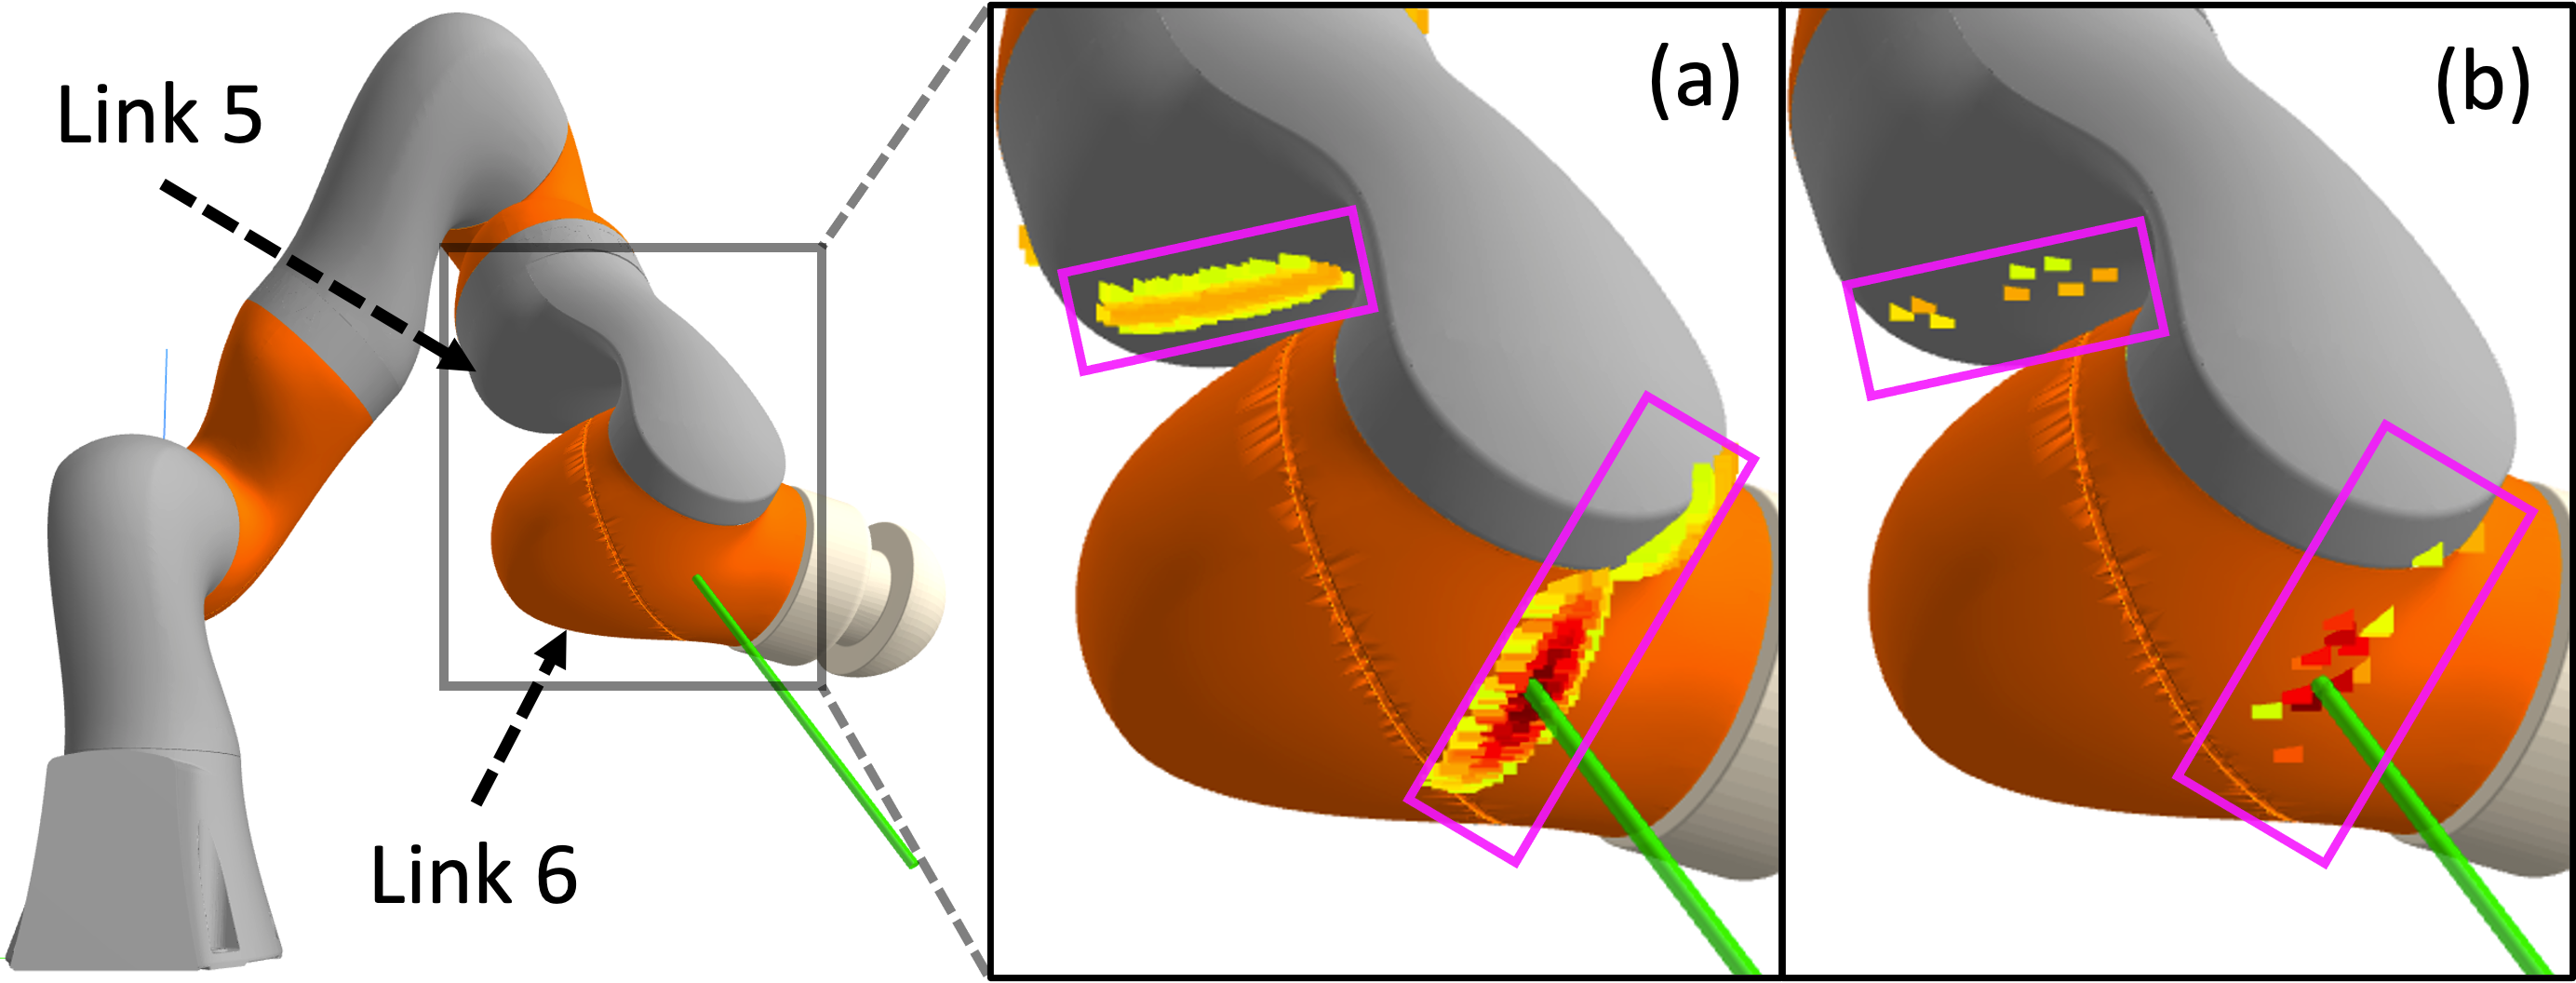
\includegraphics[width=\linewidth]{figures/05_force_from_torque/rejection_sampling.png}
    \caption{Finding elements of $P_{\epsilon}$ on link 5 and link 6 with $\epsilon=0.005$ using rejection sampling. A force of $10\mathrm{N}$ is applied to the robot along the green line. Enclosed by magenta boxes, the colored squares represent accepted samples. (\textbf{a}) Dense $P$: 491 out of 20000 samples are accepted.  (\textbf{b}) Sparse $P$: 24 out of 1000 samples are accepted.}
    \label{fig:rejection_sampling}
    \vspace{-0.6cm}
\end{figure}

\subsection{Rejection sampling + gradient descent (RSGD)\label{sec:proposed_contact_estimator}}
The high computational cost of vanilla rejection sampling, due to the high rejection rate for small $\epsilon$, can be reduced significantly by
\begin{enumerate}
\item  Generating a set of potential contact positions by rejection sampling using a sparse sample set $P$ and a large threshold $\delta$: 
\begin{equation}
P_{\delta}(q, \tauE) \coloneqq \{\pCbar \in P : l(\pCbar; q, \tauE) \leq \delta\}.
\end{equation}

\item  Running gradient descent (Algorithm \ref{algo:gradient_descent}) for every $\pCbar \in P_{\delta}(q, \tauE)$, collecting the converged points $p_{\bar{C}^\star}$ into a set of locally optimal contact position estimates: 
\begin{equation}
P^\star_{\delta}(q, \tauE) \coloneqq \{p_{\bar{C}^\star} \in \mathcal{S}\}. 
\end{equation}
Note the bar over $\bar{C}^\star$. The bar indicates that the converged point $\bar{C}^\star$ is only an estimate of the true contact point $C^\star$.
\end{enumerate}

As shown in Fig. \ref{fig:rsgd}, a large $\delta$ in Step 1 increases the acceptance rate, ensuring that $P_{\delta}$ has enough samples even if the initial sample set $P$ is sparse. Although samples in $P_{\delta}$ are spread out at the beginning, Step 2 runs them through Algorithm 1, making most of them converge to local minima of $l(\cdot)$.
\begin{algorithm}[h]
\caption{Gradient descent on manifold $\mathcal{S}$}\label{algo:gradient_descent}
\textbf{Input}: ${q}$, $\tauE$, $\pCbar$\; 
\textbf{Output}: $p_{\bar{C}^\star}$\;
\While{$\norm{\nabla_{\pCbar} l(\pCbar; q, \tauE)} > \varepsilon_G$} {
    ${t} \gets \left({I}_3 - {n}_C {n}_C^\intercal \right)\nabla_{\pCbar} l(\pCbar; q, \tauE)$ \label{algo:gradient_descent:gradient_projection}\;
    $a \gets \mathrm{LineSearch}(\pCbar, {t})$ \label{algo:gradient_descent:line_search}\;
    $\pCbar \gets \pCbar + a {t}$\;
    $\pCbar \gets \mathrm{Retract}(\pCbar, \mathcal{S})$ \label{algo:gradient_descent:retract}\;
}

$p_{\bar{C}^\star} \gets \pCbar$\;
\end{algorithm}

\begin{figure}[h]
\centering
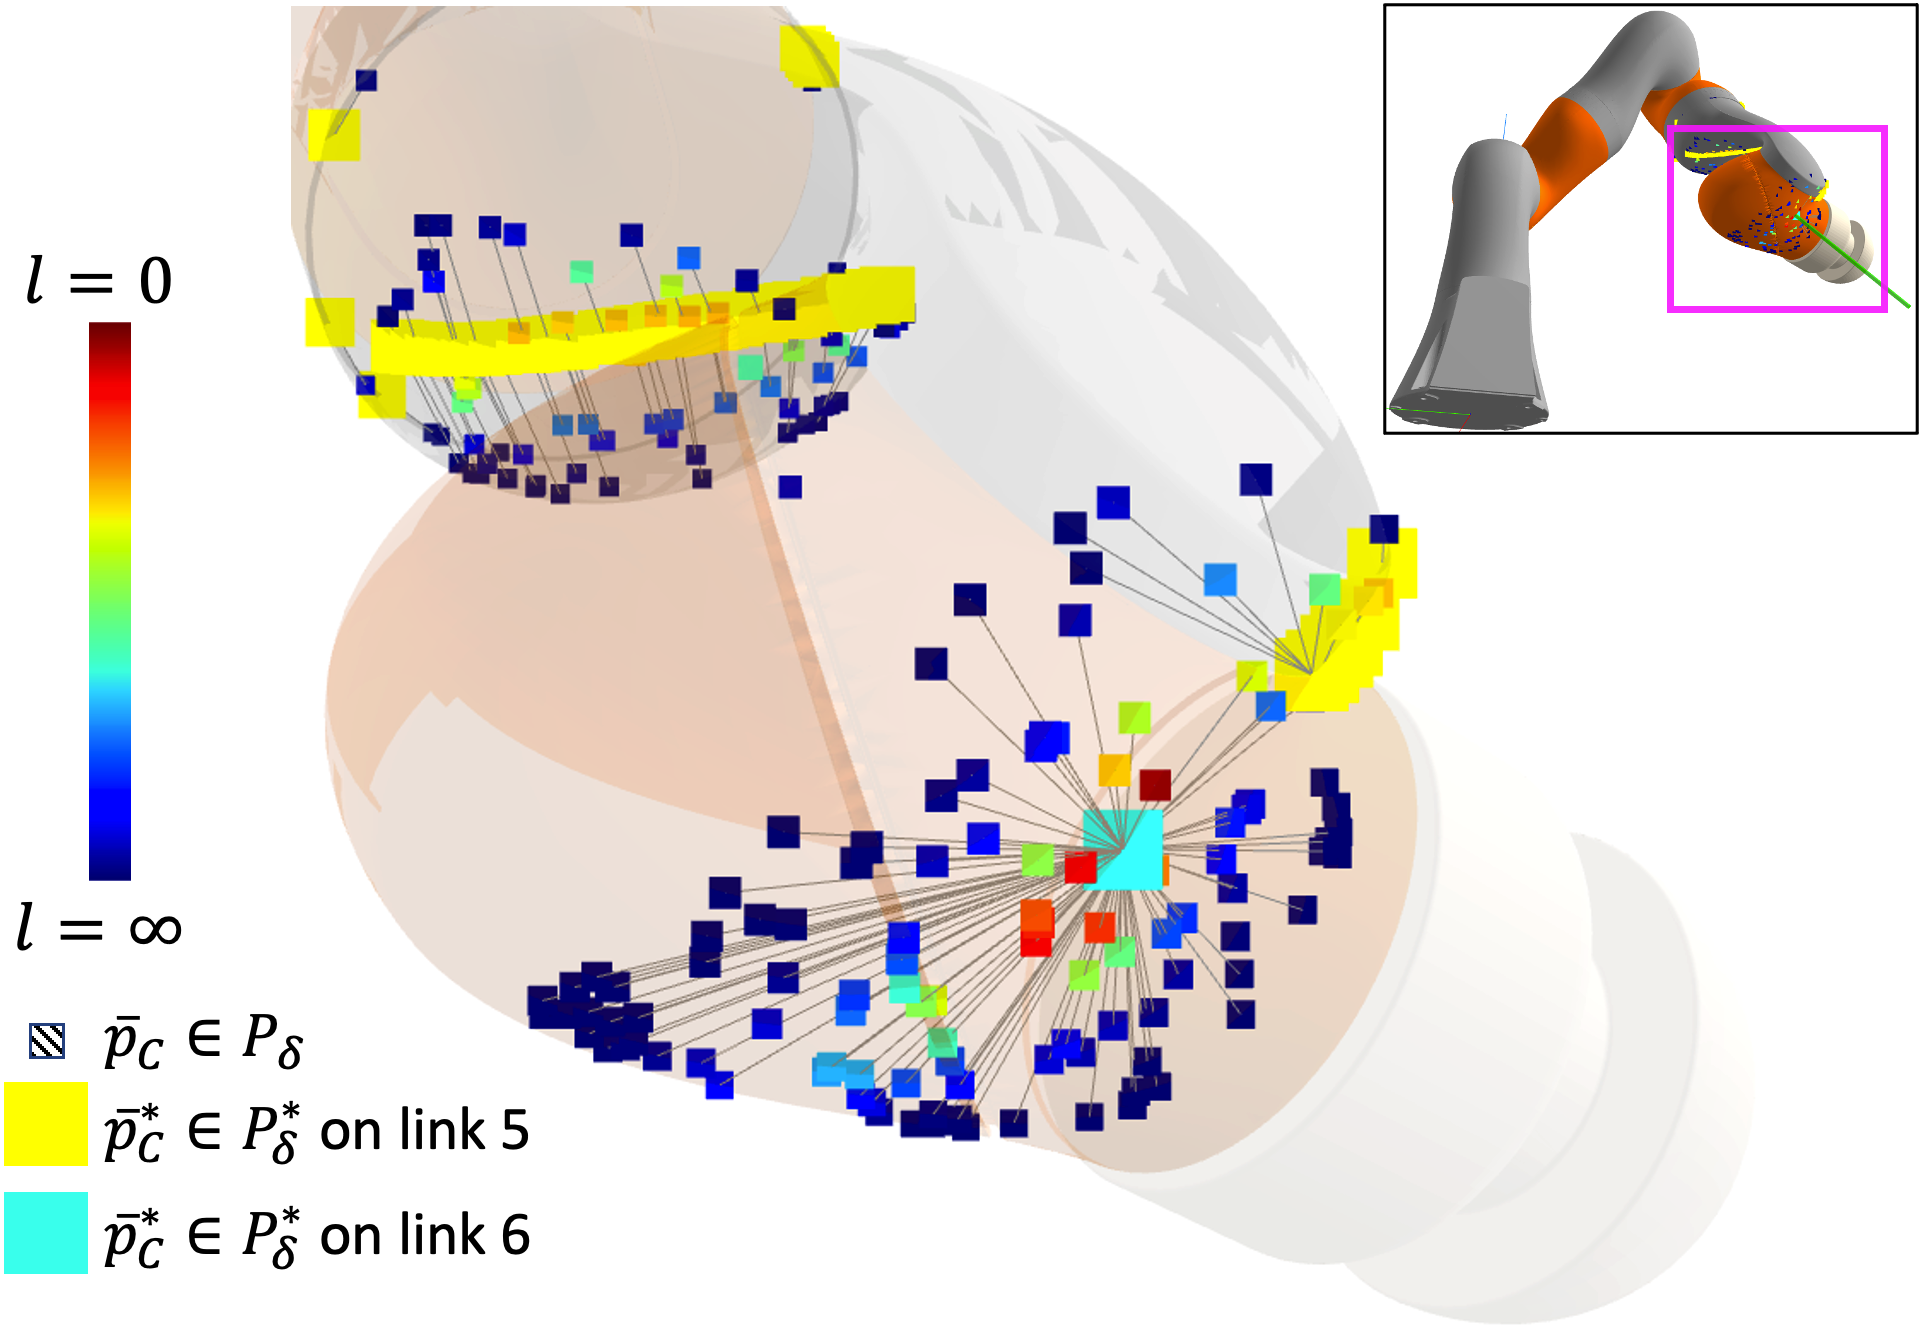
\includegraphics[width=0.9\linewidth]{figures/05_force_from_torque/rsgd.png}
\caption{Running RSGD on the same robot and contact configuration as Fig. \ref{fig:rejection_sampling}. Step 1: 175 out of 1000 samples are accepted with $\delta = 0.1$, which are shown as small squares color-coded by their residual values $l$. Step 2: 155 of the 175 samples in $P_\delta$ converge after running Algorithm 1, which are shown as large squares. Every $\pCbar \in P_\delta$ is connected by a line to the corresponding element in $P_\delta^\star$ to which it converges.}
\label{fig:rsgd}
\end{figure}

Algorithm \ref{algo:gradient_descent} is the standard Gauss-Newton method for Riemannian optimization. In Line \ref{algo:gradient_descent:gradient_projection}, the gradient $\nabla_{\pCbar} l$ is projected to the local tangent plane, which has normal ${n}_C$ and passes through $\pCbar$. In Line \ref{algo:gradient_descent:line_search}, a standard line search method is used to ensure that $l$ is decreasing after taking the gradient step $a{t}$ \cite{boyd2004convex}. In Line $\ref{algo:gradient_descent:retract}$, the new point in the local tangent plane is projected back onto $\mathcal{S}$.

Using (\ref{eq:residual_qp:qp}), the gradient $\nabla_{\pCbar} l$ can be written as 
\begin{equation}
\label{eq:l_gradient_chain_rule}
\left(\nabla_{\pCbar} l \right)^\intercal =
\frac{\partial l}{\partial \pCbar} = \frac{\partial l}{\partial \mathbf{Q}} \frac{\partial \mathbf{Q}}{\partial \pCbar} + \frac{\partial l}{\partial {b}} \frac{\partial {b}}{\partial \pCbar}
\end{equation}
where $\frac{\partial \mathbf{Q}}{\partial \pCbar}$ and $\frac{\partial {b}}{\partial \pCbar}$ can be obtained using automatic differentiation \cite{griewank1989automatic}$; \frac{\partial l}{\partial \mathbf{Q}}$ and $\frac{\partial l}{\partial {b}}$ can be obtained from differentiating the implicit function defined by the optimality condition of QP (\ref{eq:residual_qp:qp}) \cite{boot1963sensitivity}.

As shown in Fig. \ref{fig:gradient_descent}a, Algorithm 1 is effective at reducing the residual $l(\cdot)$ of samples in $P_\delta$. Note that about 60 samples converge to positions on $\mathcal{S}$ with $l = 0.003$, which is a local minimum on link 5, but not the global minimum on link 6. An example gradient descent run is shown in Fig. \ref{fig:gradient_descent}b.
\begin{figure}[h]
\centering
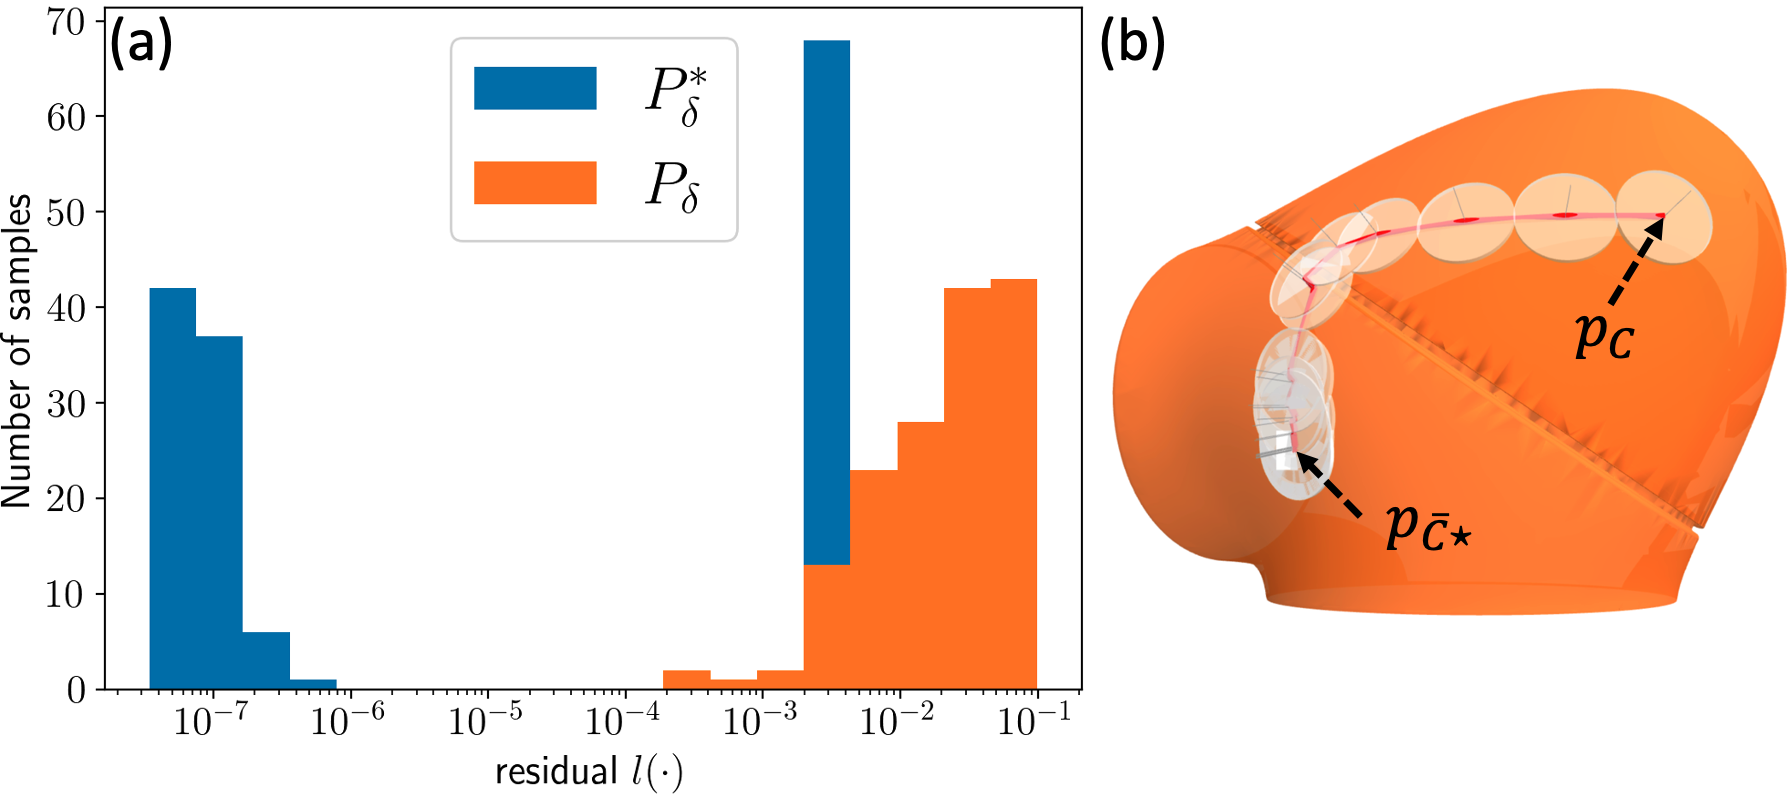
\includegraphics[width=0.85\linewidth]{figures/05_force_from_torque/gradient_descent.png}
\caption{(\textbf{a}) Distribution of residual $l(\cdot)$ of the $P_\delta$ and $P_\delta^*$ from Fig. \ref{fig:rsgd}. (\textbf{b}) A gradient descent run on link 6 of IIWA. Algorithm \ref{algo:gradient_descent} starts at $\pCbar \in \mathcal{S}$ and converges to $p_{\bar{C}^\star}$. Red lines represent the path taken by gradient descent. White translucent disks represent local tangent planes. }
\label{fig:gradient_descent}
\end{figure}

The ability of an approach such as RSGD to find all local minima depends on two factors: the sampling strategy and the convergence properties of gradient descent. 
% Concerning the former, 
By construction the entire surface of the robot is contained with the support of the distribution of the sampling procedure.
As such, for every local minimum that has a non-measure-zero region of attraction, the probability that we draw a sample in that region and converge to the minimum in non-zero.  
Characterizing these regions of attraction, however, is more challenging, and one cannot rule out, e.g. saddle points and limit cycles. 
Nevertheless, empirically, we observe that the algorithm succeeds in finding all local minima for sufficiently dense sampling.

%%%%%%%%%%%%%%%%%%%%%%%%%%%%%%%%%%%%%%%%%%%%%%%%%%%%%%%%%%%%%%%%%%%%%%%%%%%%%%%%
\section{Active contact discrimination}
In the event that RSGD returns multiple (possible) contacts, some form of active exploration may be desirable to discriminate the true contact from the spurious.
Assuming contact with a static object, that will remain (approximately) in place irrespective of the robot's motion, a simple strategy to falsify a spurious contact is to move the robot so as to break contact (pull away) at that location; if residual torque remains, then this cannot have been the true contact (assuming no additional contacts were introduced during the robot's motion). 
Similarly, the robot motion may preserve (push into) a possible contact; if the residual torque vanishes, then this (spurious) contact is falsified. 
Given $\numcontact$ possible contacts 
$\lbrace \contact{i}\rbrace_{i=1}^\numcontact$, 
rather than test each (possible) contact individually, it is more efficient to ``pull away from'' $\lfloor{\numcontact/2}\rfloor$ such contacts, and ``push into'' the other $\lceil{\numcontact/2}\rceil$, thereby falsifying half of the contacts with each change of robot pose. 
The following program searches for such a change in pose, $\dq\in\real^\numjoints$.
\begin{subequations}
\label{eq:miqp}
\begin{align}
& \min_{\dq, \ \pull\in\binary^\numcontact} \ |{\sum}_{i=1}^\numcontact \pull_i - \lfloor{\numcontact/2}\rfloor | \label{eq:miqp:cost} \\
& \normal{i}\transp\jackobian{i}\dq \leq \maxpush - (\maxpush + \minpull)\pull_i, \ i = 1,\dots,\numcontact \label{eq:miqp:pull} \\
& \normal{i}\transp\jackobian{i}\dq \geq \minpush - (\minpush + \maxpull)\pull_i, \ i = 1,\dots,\numcontact  \label{eq:miqp:push} \\
& | (I - \normal{i}\normal{i}\transp)\jackobian{i}\dq | \leq \maxrad, \ i = 1,\dots,\numcontact \label{eq:miqp:orth} \\
& |\dq| \leq \dqmax\ones. \label{eq:miqp:lim}
%\ i = 1,\dots,\numcontact.
\end{align}
\end{subequations}
Here, $\pull\in\binary^\numcontact$ represents the decision(s) to pull away ($\pull_i=1$) or push into ($\pull_i=0$) the $i$th contact.
The objective \eqref{eq:miqp:cost} attempts to push into as close to half ($\lfloor{\numcontact/2}\rfloor$) of the contacts as possible.
The constraints \eqref{eq:miqp:pull} and \eqref{eq:miqp:push} require that, e.g., a ``pull away'' moves the $i$th possible contact point (on the robot) at least $\minpull$, but at most $\maxpull$, in the opposite direction to the outward facing surface normal $\normal{i}$, assuming a linearized relationship between the change in position and change in pose, 
$\dpos\approx\jackobian{i}\dq$.
Constraint \eqref{eq:miqp:orth} restricts the motion (of each contact point) close to the corresponding surface normal, to minimize the chance of introducing new contacts after the change in pose.
Constraint \eqref{eq:miqp:lim} restricts the change in each joint angle.
An example of this method in action is shown in Fig. \ref{fig:active_contact_discrimination}.
\begin{figure}[h]
\centering
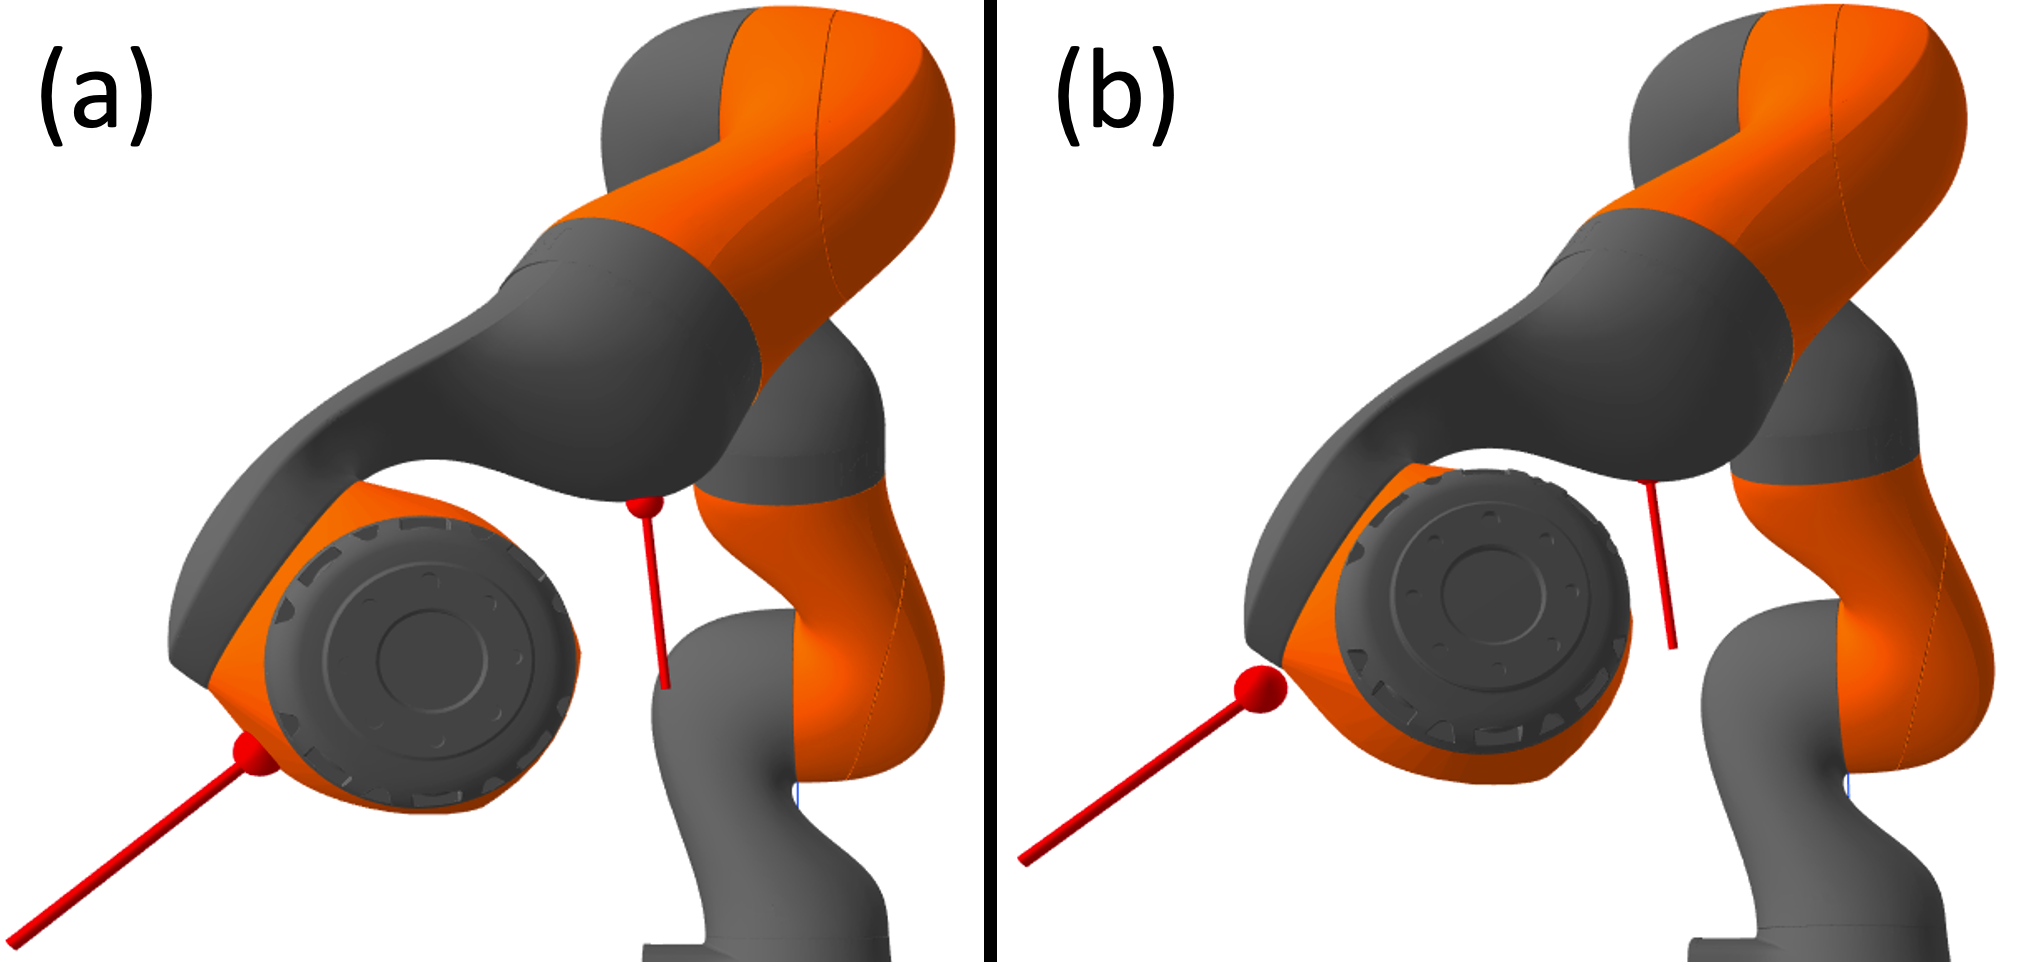
\includegraphics[width=0.75\linewidth]{figures/05_force_from_torque/active_contact_discrimination.png}
\caption{(\textbf{a}) Two possible contact positions to disambiguate. The centers of the small red spheres are coincident with the candidate contact positions. (\textbf{b}) Solving (\ref{eq:miqp}) finds a motion that pulls away from the contact on link 6 and pushes into the contact on link 5. }
\label{fig:active_contact_discrimination}
\end{figure}

There is no guarantee that this simple discrimination strategy will falsify all spurious contacts; success depends on problem specifics, e.g. robot pose, robot geometry, and the contact locations.
In particular, \eqref{eq:miqp} may return \texttt{infeasible}, or $\pull\equiv\ones$ ($\pull\equiv\mathbf{0}$) (i.e. pull/push on all contacts, which gathers no useful information). 
However, problem \eqref{eq:miqp} is a (convex) mixed-integer linear program (MILP) that can be efficiently solved to global optimality by commercial solvers. 
This means that, in the event of failure, we have a certificate that no such (sequence of) discriminating actions $\dq$ exist, at least not without relaxing the constraints \eqref{eq:miqp:pull}-\eqref{eq:miqp:lim}, or abandoning the linearized model and resorting to 
% (computationally more expensive) 
nonlinear motion planning.  

%%%%%%%%%%%%%%%%%%%%%%%%%%%%%%%%%%%%%%%%%%%%%%%%%%%%%%%%%%%%%%%%%%%%%%%%%%%%%%%%
\section{Implementation}
RSGD requires a lot more computation than existing methods. Nevertheless, by leveraging efficient open-source libraries, our implementation can run at real-time rates on a single CPU thread.

Fig. \ref{fig:run_time} shows the run-time breakdown of a typical iteration of RSGD, collected on a Mac mini with Intel i7-8700B CPU and 64GB of RAM. In Step 1, the residual $l(\cdot)$ is computed for 1000 points drawn uniformly from $S$, of which 184 points satisfy $l < \delta$. In Step 2, Algorithm \ref{algo:gradient_descent} is run on each of the 184 points until convergence, or until the limit on gradient steps is reached.
\begin{figure}[h]
\centering
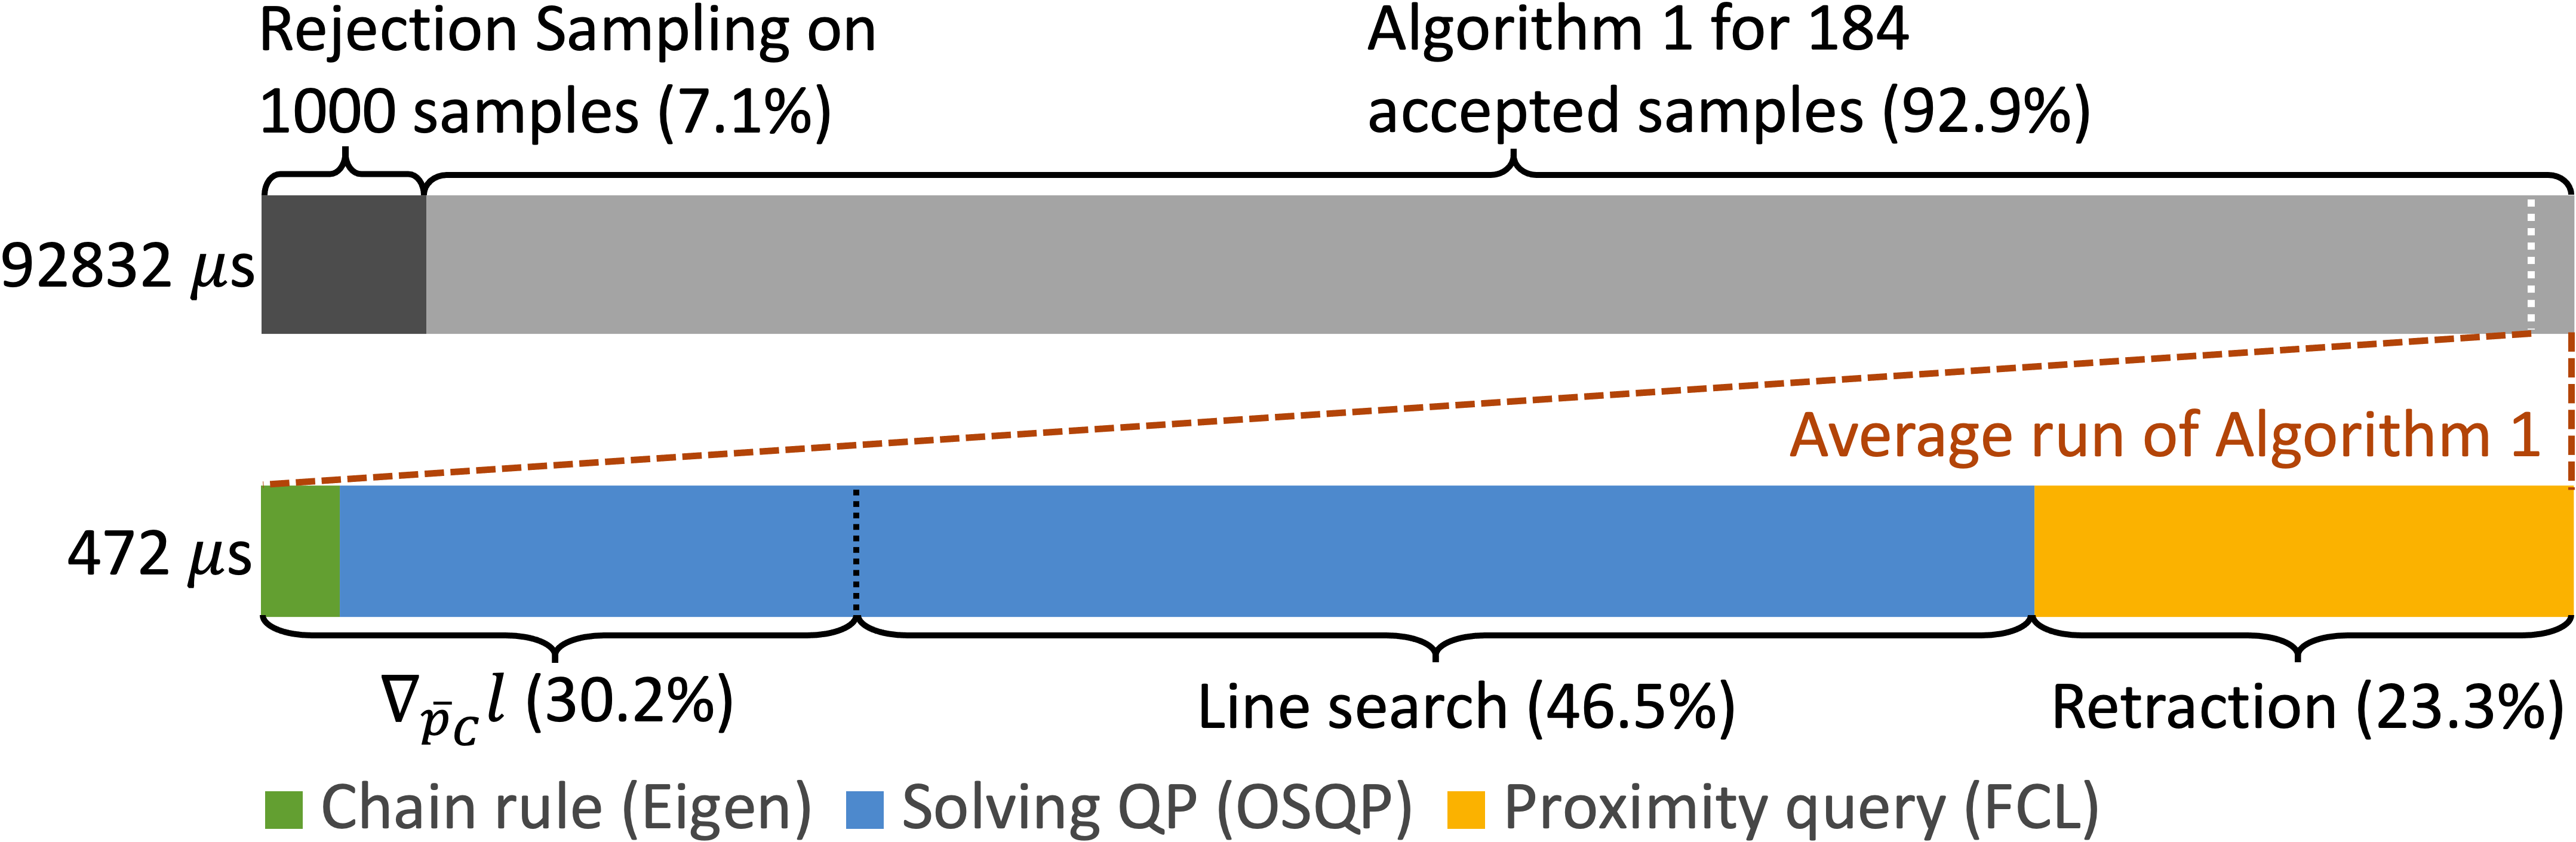
\includegraphics[width=0.95\linewidth]{figures/05_force_from_torque/run_time.png}
\caption{Run-time breakdown of a typical iteration of RSGD.}
\label{fig:run_time}
\end{figure}

As most of the time is spent on running Algorithm \ref{algo:gradient_descent} for accepted samples in $P_\delta$, how long one iteration of RSGD takes is almost linearly proportional to $|P_\delta|$. In this case, $|P_\delta|=184$ leaves RSGD running at roughly 10Hz. This can be improved, for instance, by using a sparser $P$, putting an upper bound on $|P_\delta|$, using more CPU threads, or a combination of these strategies. 

An average run of Algorithm \ref{algo:gradient_descent} takes $472 \mu s$. The most frequently-used atomic operation is computing the residual $l(\cdot)$, which involves solving QP (\ref{eq:residual_qp:qp}). In every gradient step, $l(\cdot)$ needs to be computed once to evaluate the gradient $\nabla_{\pCbar} l(\cdot)$, and a couple more times by line search. Moreover, $l(\cdot)$ is also computed for every sample in $P$ in the earlier rejection sampling step. The lightweight QP solver OSQP\cite{stellato2020osqp} allows us to compute $l(\cdot)$ quickly: it takes $6\mu s$ on average to solve QP (\ref{eq:residual_qp:qp}). 

Retracting points back onto the robot surface $\mathcal{S}$ is the second most time-consuming operation in Algorithm \ref{algo:gradient_descent}. With the robot surface $\mathcal{S}$ represented by triangle meshes, retraction can be done efficiently by a mature proximity query routine implemented in the Flexible Collision Library (FCL) \cite{pan2012fcl}. 

The chain rule for computing $\nabla_{\pCbar} l(\cdot)$ in (\ref{eq:l_gradient_chain_rule}) is implemented with Eigen \cite{eigenweb}, which takes only 2\% of the total time needed for Algorithm \ref{algo:gradient_descent} to converge.

Algorithm \ref{algo:gradient_descent} may fail to converge if gradient descent passes through a region of $\mathcal{S}$ with almost discontinuous surface normal, e.g. a groove or an engraved letter. Proximity queries also occasionally return a point off the mesh, throwing gradient descent off its track. Nonetheless, such failures are relatively rare and easy to detect and reject when they do occur.

Concerning the active contact discrimination, although complexity of the MILP is exponential in the number of contact locations to be falsified, moderate-size problems can be solved efficiently with SOTA solvers, such as GUROBI \cite{gurobi}; e.g., a problem with $\numcontact=10$ contacts can be solved in approximately 5ms.


\section{Conclusion}
With a detailed analysis on two notions of contact detectability, we have demonstrated that a contact estimate from joint torque measurements typically consists of more than one possible contact positions, which are the global minima of the residual function $l(\cdot)$. 
Finding all global minima of $l(\cdot)$ is generally hard, but the proposed RSGD estimator empirically locates all local minima of $l(\cdot)$. 
Considering that joint torque measurements are inherently noisy, being able to find contact points with a small but positive residual could actually be beneficial. 
We have also provided a strategy to search for small robot motions which falsify as many spurious contact positions found by RSGD as possible. Moreover, when this strategy fails, it provides a certificate that no other small motion can do better.

On a robot that streams joint angle and residual torque ($\tauE$) signals, such as the KUKA IIWA, deploying RSGD is expected to be straightforward. Nevertheless, pre-processing of the raw $\tauE$ signal provided by the robot's driver, which filters out noise and ensures that the signal is unbiased, will probably be necessary.
